\chapter{Material and Methods}\label{cap:studyOfTools}

This chapter endeavors to elucidate the technological tools and methodologies deployed across various stages of this project’s development. Specifically, in Section \ref{section:imageProcessing}, an introduction to certain image processing methodologies, notably Gaussian filtering and Canny edge detection, is presented. Both these image processing techniques form the crux of algorithms employed for acquiring distinct edges of wood pieces. This, in turn, facilitates the automatic classification of the geometries of the wood leftovers.

In Section \ref{section: System}, the devices employed in the traceability solution proposed for wood leftovers are delineated. Furthermore, in Section \ref{section:comunication}, the communication methodologies between the various services and devices that constitute the solution are explicated. Such information is vital for the definition of the system's architecture.
 
 
In Section \ref{section:conceptulaDataModel}, a conceptual data model is developed, which is integral for an in-depth analysis of the company's operations and for crafting an architecture tailored to its specific requirements. Additionally, aspects related to the databases employed are elucidated in Section \ref{section:mmDataBase}, furnishing insights regarding the tools that were selected for the construction of the system's overall architecture.

Moving on to Section \ref{section:security}, crucial aspects regarding security that were employed in the overall system architecture are delineated.

The tools employed for file sharing are defined in Section \ref{section:fileSharing}, and Section \ref{section:fileSharing-webserver} details the necessary aspects and the servers used for potential project monitoring.

Section \ref{section:ProjectTraceability} addresses the methodological aspects involved in project traceability, and finally, Section \ref{section:LeftoverTraceability} describes the methods employed for leftover traceability.

\section{Digital Image Processing}\label{section:imageProcessing}

Digital image processing is a field that addresses the manipulation, analysis, and interpretation of digital images, which are discrete two-dimensional functions, $f(x_i, y_i)$, composed of elements called pixels. This discipline encompasses a wide spectrum of applications and is related to areas such as image analysis and computer vision. Digital image processing can be divided into low, medium, and high-level processes. Low-level processes involve pre-processing and image enhancement, while medium-level processes deal with segmentation, description, and classification of objects. On the other hand, high-level processes seek to make sense of sets of recognized objects and perform cognitive functions associated with vision. Digital image processing encompasses processes that work with image inputs and outputs and also processes that extract attributes from images, including the recognition of individual objects, successfully applied in various areas of social and economic value \cite{gonzalez_rafael_c_digital_2018}.

In this multidisciplinary field, a wide range of techniques and algorithms is employed to optimize image quality, enhance features of interest, and facilitate the extraction of valuable information. Such approaches can be applied in various contexts, ranging from improving the quality of images obtained by digital photographic devices to the analysis of data in images for specific applications \cite{ekstrom2012}.

However, as reported by \textcite{mcandrew2004introduction}, image processing addresses two distinct and fundamental aspects:
\begin{enumerate}
\item Enhance the pictorial information for human interpretation.
\item Make the image more suitable for autonomous machine perception.
\end{enumerate}

The first aspect refers to enhancing the pictorial information of an image for human interpretation, which involves improving the visual appearance of the image. The second aspect aims to make the image more suitable for autonomous machine perception, which implies simplifying and organizing the image efficiently. These two conditions require distinct and specialized procedures, and a procedure that satisfies one condition may not necessarily satisfy the other. As can be seen in figure \ref{fig:imageProcessingExample}, despite the processed image presenting greater significance for a contour analysis, it may not have an attractive aspect to the human eye \cite{mcandrew2004introduction}.



Additionally, image processing plays a crucial role in the development of computer vision systems and machine learning, allowing electronic devices and machines to interpret and understand visual information in a manner analogous to human perception. This ability to process and analyze images is essential for devising innovative solutions in areas such as robotics, industrial automation, security and surveillance, facial recognition, among others.

In summary, image processing constitutes a comprehensive and multidisciplinary field of study, encompassing knowledge from computer science and engineering, aiming to improve the quality of digital images and extract relevant information for a wide range of applications. Through the application of advanced techniques and specialized algorithms, image processing significantly contributes to the progress of computer vision and machine learning, driving innovation and technological development in various sectors.


\subsection{Gaussian Filtering}

One of the critical steps developed in this project is the ability to observe the geometry of a part, and in order to achieve this, it is necessary to apply the Gaussian filter, which will be explained in the following section.

Applying a filter to an image implies performing a convolution operation. In the continuous context and with a single variable in the domain, this operation can be represented by the equation \ref{eq:convolution} \cite{spiegel_schaums_1974}. However, when working with digital images, it is common to employ an adaptation of this equation for discrete media in a two-dimensional domain, which makes use of a base matrix, called a kernel, as illustrated in the equation \ref{eq:convolution-discreet} \cite{gonzalez_rafael_c_digital_2018}. The kernel is used to assign weights to neighboring points of a specific point in the image, modifying their values and resulting in an image with altered pixels. During convolution, the kernel is applied to each point in the image, multiplying its weights by the values of adjacent pixels, see image \ref{fig:kernel-convolution}.

\begin{equation}
(f * g)(t) = \int_{-\infty}^{\infty} f(\tau) \cdot g(t-\tau) d\tau
\label{eq:convolution}
\end{equation}

\begin{equation}
(f * w)(x_i, y_i) = \sum_{s=-a}^{a} \sum_{t=-b}^{b} f(x_i +s, y_i +t) \cdot w(s, t) \quad \forall i \in \mathbb{N}
\label{eq:convolution-discreet}
\end{equation}\\


\begin{figure}[ht!]
\centering
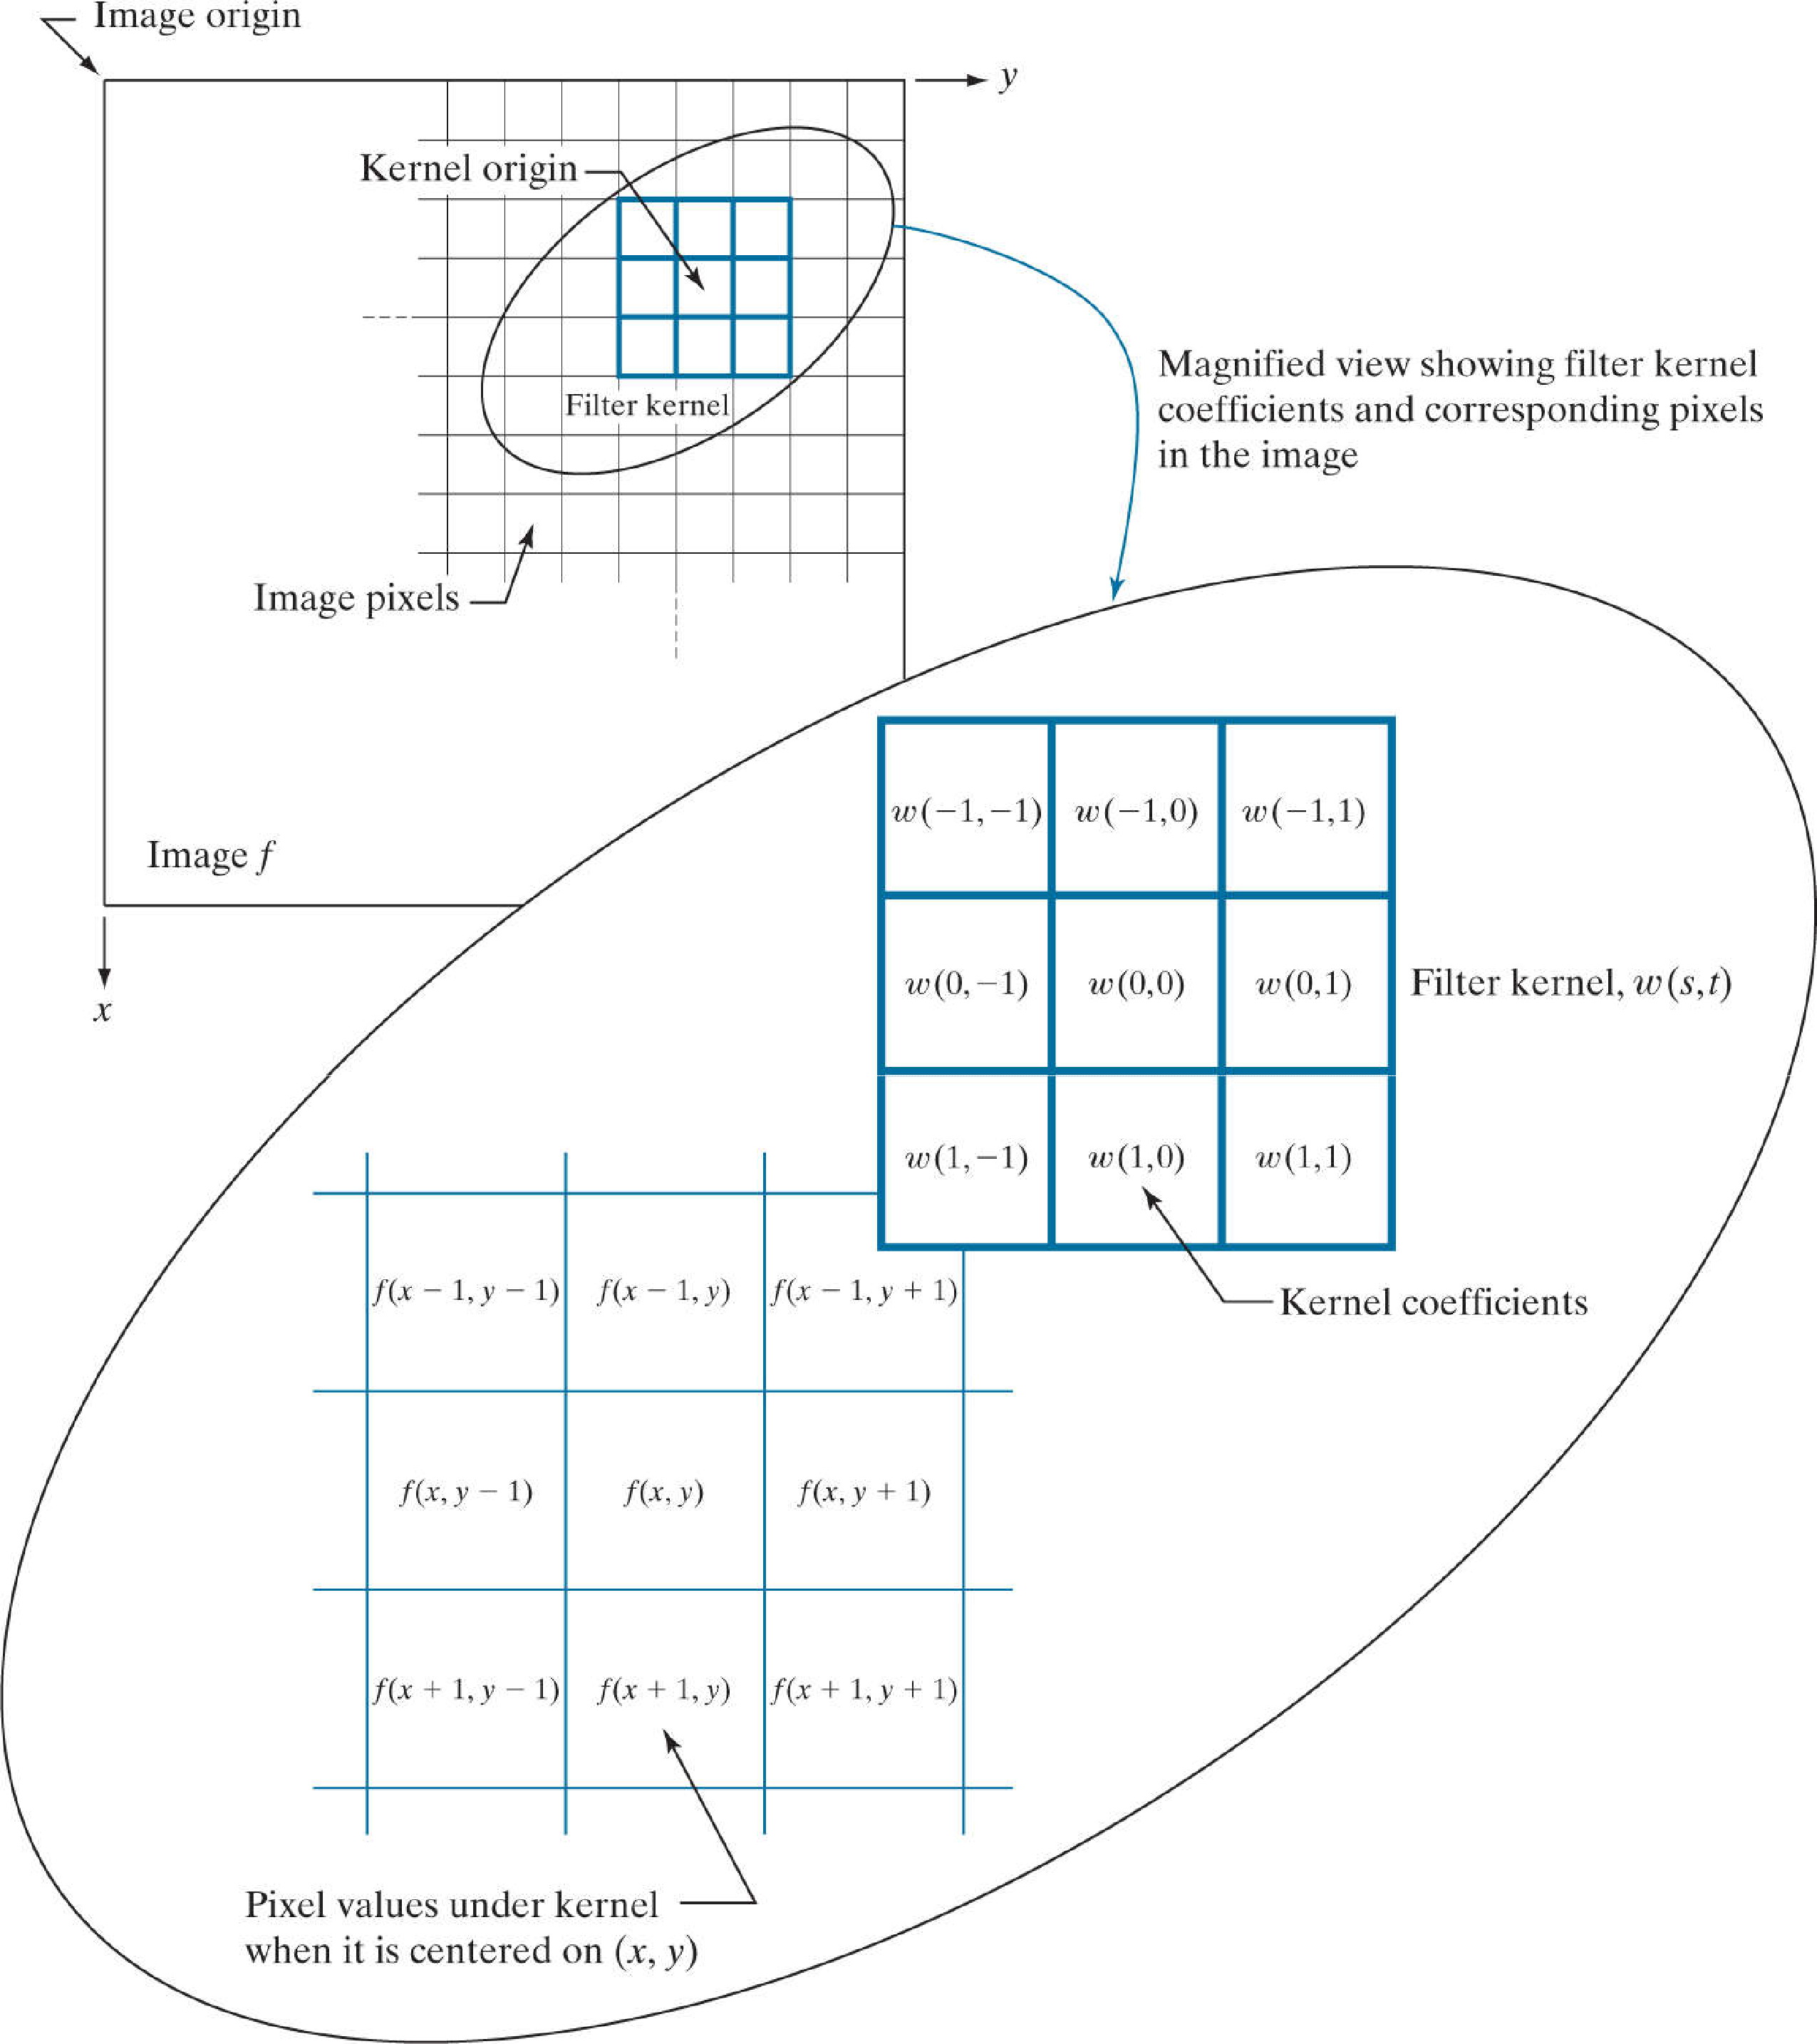
\includegraphics[width=.65\linewidth]{images/Development/chap3/kernel.png}
\caption{Kernel convolution representation on a digital image. Source: \cite{gonzalez_rafael_c_digital_2018}.}
\label{fig:kernel-convolution}
\end{figure}



The linear spatial filters are widely used and employ a kernel that performs the sum of products between the original image and the kernel itself, as shown in Figure \ref{fig:kernel-transformation}. The size of the kernel defines the neighborhood of operation, while its coefficients determine the nature of the filter. It is worth noting that different kernels can be applied for different purposes, such as enhancing sharpness, highlighting details, or detecting edges \cite{gonzalez_rafael_c_digital_2018}.



Moreover, various types of filters can be combined to achieve more sophisticated results. For example, smoothing and enhancement filters can be used together to produce sharper and more detailed images \cite{mcandrew2004introduction}. The process of applying filters can be repeated several times until the desired result is obtained; however, it is essential to consider that excessive use of filters can result in information loss and the presence of artifacts in the final image.

Filters are characterized by the dimension of the kernel and their associated weights, establishing the nature and behavior of the filter. The kernel dimension has a considerable impact on the final result of the filtering, defining the number of adjacent pixels considered during the convolution operation. Larger kernels promote a more pronounced smoothing effect and noise reduction, although they can lead to loss of fine details, while smaller kernels enable a more pronounced selective effect and preservation of fine details, but with greater sensitivity to noise presence. The distribution of kernel weights is another crucial factor that influences the filter's performance. An example is the case where a bell curve is used, as shown in Figure \ref{fig:gaussian3d}, to establish the relationship of weights $w(s, t)$. The Gaussian distribution is commonly used for this purpose, which is an exponential function that reaches its maximum at the central point of the kernel and rapidly decreases towards the edges, as shown in Equation \ref{eq:gaussian-distribuition}. This means that pixels closer to the center of the kernel will have more weight than pixels farther away, resulting in more efficient smoothing without losing fine details. Therefore, the choice of kernel and weight distribution is crucial to obtain appropriate results in image processing \cite{gonzalez_rafael_c_digital_2018, mcandrew2004introduction, DHAEYER1989}.

\begin{equation}
    w(s,t) = G(s, t) = K e^{-\frac{s^2 + t^2}{\sigma^2}} \quad  :\ K \in \mathbb{R}
    \label{eq:gaussian-distribuition}
\end{equation}

\begin{figure}[h!]
\centering
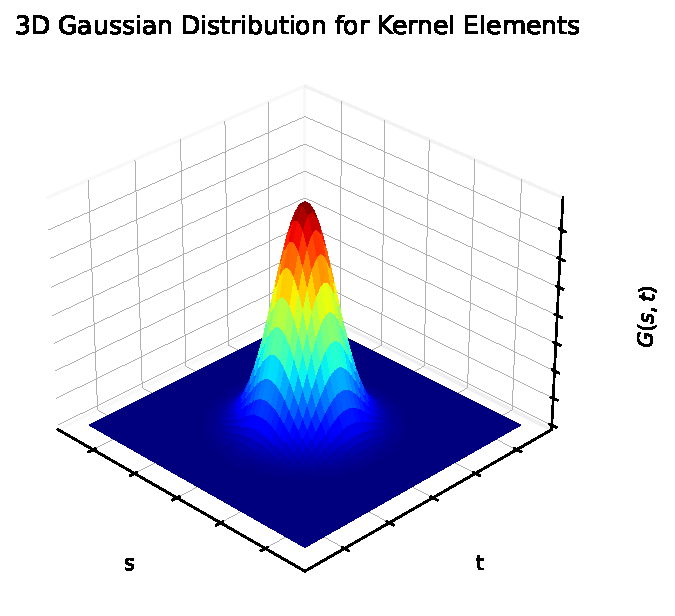
\includegraphics[width=.65\linewidth]{images/Development/chap3/gaussian_3d_plot.pdf}
\caption{Gaussian distribution.}
\label{fig:gaussian3d}
\end{figure}


The appropriate selection of the Gaussian kernel dimension is an essential aspect in image processing. Often, a kernel size that does not exceed $6\sigma$ is adopted, as values beyond $3\sigma$ from the center become practically irrelevant to the final result. This phenomenon arises from the fact that the Gaussian function has significantly reduced values at a distance greater than $3\sigma$ from its center, making them less important for filtering. Opting for a kernel of suitable dimensions is crucial to ensure an optimal balance between computational efficiency and the quality of the filtering process \cite{gonzalez_rafael_c_digital_2018}.



\subsection{Canny Edge Detection}\label{subsection:Canny-edge-detection}

Just as the Gaussian filter is used to remove noise from the image, the Canny filter is employed to detect edges. This process is essential for obtaining the geometries of the leftover materials and thereby automating the measurement process of a remnant. The fallowing section will explain this process. 

The study of vertex detection is not a recent research area in science. In the 1960s, researchers \textcite{hubel1968receptive} \cite{hubel1962} conducted pioneering studies to understand the process of vertex detection at the biological level, conducting experiments with monkeys and cats. Later, in the 1970s, researchers \textcite{daniel1971} attempted to mathematically model the perception of vertices by the cerebral cortex, using Fourier Series for this purpose.

However, it was with the popularization of digital images in the 1980s that vertex detection gained more prominence and practical applicability. It was in this context that \textcite{marr1980theory} developed a mathematical analysis for image processing, with the aim of identifying vertices. In this study, the authors used the Laplacian applied to the Gaussian distribution. The contribution of these authors provided a solid foundation for subsequent studies in this area.

Subsequently, \textcite{canny1986} made significant advances in the vertex detection process, optimizing the initial process developed for vertex processing. As a result of their work, a widely known and used filter emerged, which was named the "Canny Filter". This filter became a reference in the field of image processing, offering an effective and robust approach for the precise detection of vertices in various applications \cite{ding_canny_2001}.

Vertices are a characteristic present in images, representing regions where two groups of pixels with similar tones differ. In other words, they are areas where there are abrupt changes in pixel intensity. In real-world images, edges often exhibit blur and display a smooth transition, resulting in thicker edge positions due to the blurring effect. However, from a mathematical point of view, the derivative of a smooth transition is a step function, and the first-order derivative is zero in regions with constant intensity levels and has nonzero values throughout the transition region \cite{Chaple2015}. Therefore, the magnitude of the first-order derivative can be used to detect edges \cite{gonzalez_rafael_c_digital_2018}. Figure \ref{fig: imageBoundary} visually reveals these discussed characteristics.

\begin{figure}[ht!]
\centering
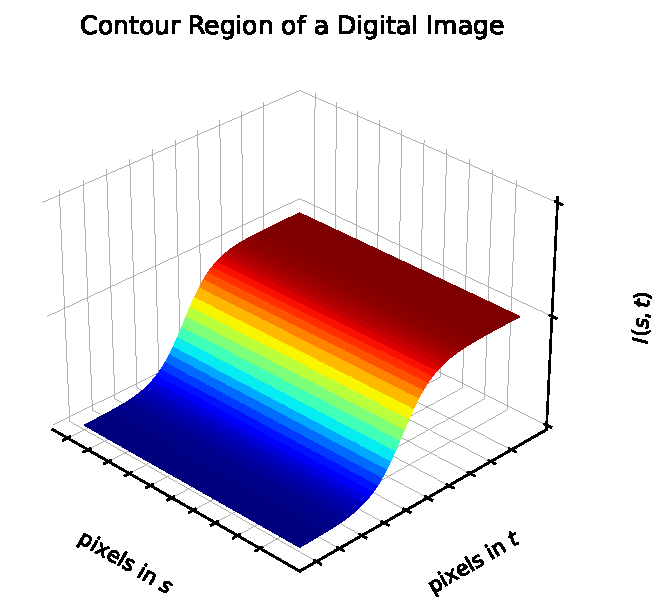
\includegraphics[width=.65\linewidth]{images/Development/chap3/chart.pdf}
\caption{Graphical depiction of a vertex region wherein the digital image $I(s, t)$ exhibits a variation in the intensity of its pixels. Adapted from: \cite{marr1980theory}.}
\label{fig: imageBoundary}
\end{figure}


Thus, as an image represents a function with a domain in two-dimensional space \cite{marr1980theory}, we can calculate its variation using the differential operator nabla \cite{Zhang2020}. The nabla operator applied to the function \(f(x, y)\) is represented by the following equation:


\begin{equation}
    \nabla f(x, y) = \frac{\partial f}{\partial x} \mathbf{i} + \frac{\partial f}{\partial y} \mathbf{j}
\end{equation}

In the context of digital images, it is necessary to adapt this operator. One of the approaches used is the Prewitt-Sobel operator.

The Prewitt operator was initially proposed as a type of edge detection that uses a first-order differential operator. It calculates the intensity difference between neighboring pixels in the vertical and horizontal directions. At edges, this mathematical object is capable of detecting extremes, removing false edges, and smoothing noise \cite{Zhang2020, prewitt1970object}. It can be obtained in the form of equations \eqref{eq:py} and \eqref{eq:px}. These equations represent the kernels of the Prewitt operator that are used to convolve a digital image.

\begin{equation}
    P_t= \
\begin{bmatrix}
-1 & 0 & 1 \\
-1 & 0 & 1 \\
-1 & 0 & 1 \\
\end{bmatrix} 
* I(s, t)
\label{eq:py}
\end{equation}
\begin{equation}
    P_s = 
\begin{bmatrix}
-1 & -1 & -1 \\
0 & 0 & 0 \\
1 & 1 & 1 \\
\end{bmatrix}
 * I(s, t)
\label{eq:px}
\end{equation}

Subsequently, the Sobel operator was developed as an improvement over the Prewitt operator. It introduces a weight of 2 on the central coefficient of the mask, as shown in equations \eqref{eq:gs} and \eqref{eq:gt}. This allows for better noise suppression compared to the Prewitt operator \cite{Zhang2020}. Thus, the Prewitt-Sobel operator is an evolution of the Prewitt operator, incorporating the enhancements introduced by the Sobel operator. The Prewitt-Sobel operator is defined as follows:

\begin{equation}
G_s = \begin{bmatrix}
-1 & 0 & 1 \\
-2 & 0 & 2 \\
-1 & 0 & 1
\end{bmatrix} * I(s, t)
\label{eq:gs}
\end{equation}

\begin{equation}
G_t= \begin{bmatrix}
-1 & -2 & -1 \\
0 & 0 & 0 \\
1 & 2 & 1
\end{bmatrix} * I(s, t)
\label{eq:gt}
\end{equation}
Where \(G_s\) and \(G_t\) are the convolution responses with the Sobel masks in the horizontal and vertical directions, respectively. The process of applying these masks can be observed in Figure \ref{fig: sobelApplyed}.
\begin{figure}[ht!]
\centering
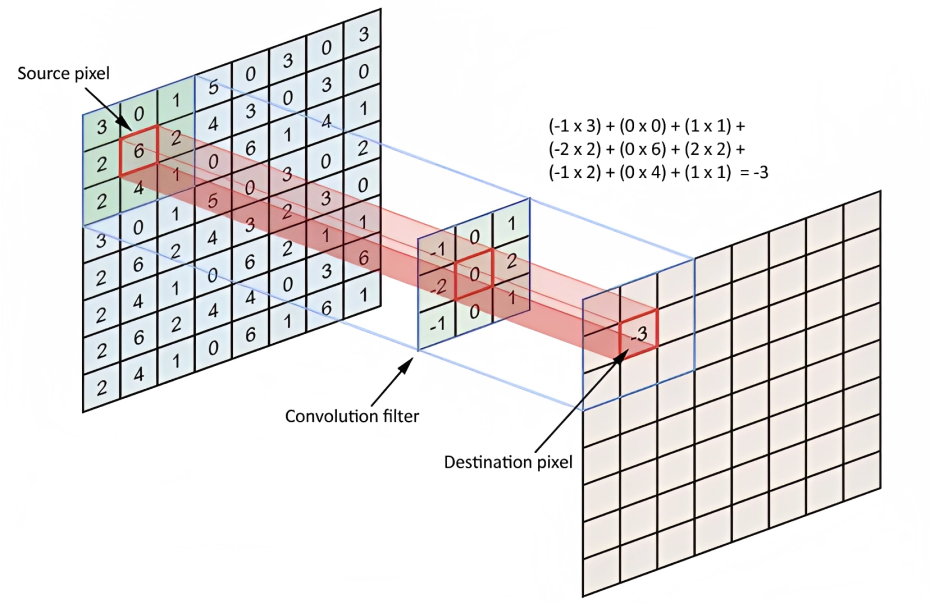
\includegraphics[width=.65\linewidth]{images/Development/chap3/mask.png}
\caption{The image depicts the application of the Sobel operator to an image, which is a commonly used technique for edge detection. Source: \cite{Matthew2020}.}
\label{fig: sobelApplyed}
\end{figure}

Thus, the intensity and direction of the gradient can be obtained through Equations \eqref{eq:arctG} and \eqref{eq:mapprox} \cite{gonzalez_rafael_c_digital_2018, Zhang2020}.

\begin{equation}
    \theta = \arctan \left( \frac{{G_t}}{{G_s}} \right)
    \label{eq:arctG}
\end{equation}

\begin{equation}
    \text{{M}} = \sqrt{{G_s^2 + G_t^2}}
\end{equation}
Which can be approximated in the equation \ref{eq:mapprox} \cite{gonzalez_rafael_c_digital_2018}: 
\begin{equation}
    \text{{M}} \approx \|G_s\| + \|G_t\| 
    \label{eq:mapprox}
\end{equation}

After calculating the gradients, considering their respective directions and magnitudes, non-maximum suppression is implemented. This technique aims to identify and preserve those local maximum points that typically align with the edges of an image. The methodology for this process, although intricate, can be described in an accessible manner. The first step is to determine the direction in which the maximum gradient variation occurs in a specific region. Next, the point of maximum intensity along this direction is identified. Among the various possible points, only this point of maximum intensity is retained, resulting in the elimination of other points that do not correspond to local maxima. Figure \ref{fig: suppression} can be used to illustrate this situation. Let's consider point A located on the edge (vertical direction) of the image. The gradient direction, in this case, is normal to the edge. Points B and C, on the other hand, lie in the gradient directions. Thus, point A is compared to points B and C to determine if it constitutes a local maximum. If this condition is satisfied, point A is considered for the subsequent step. Otherwise, it is suppressed (assigned a value of zero) \cite{canny_opencv_nodate}.

\begin{figure}[ht!]
\centering
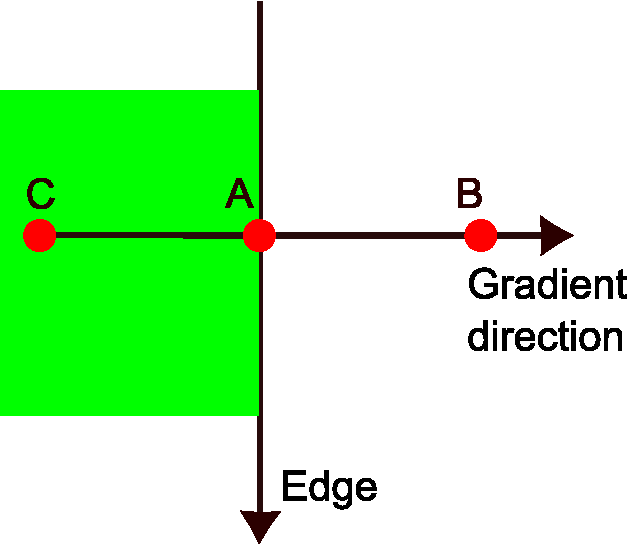
\includegraphics[width=.65\linewidth]{images/Development/chap3/opencv.pdf}
\caption{Suppression of non-maximums. Adapted from: \cite{canny_opencv_nodate}}
\label{fig: suppression}
\end{figure}
As a final step, the edge detection process aims to identify truly significant edges, distinguishing them from those that are considered less relevant or false. To achieve this, two threshold values, minVal and maxVal, are established, as shown in Figure \ref{fig: hysteresis}. Edges that exhibit intensity gradients exceeding the maxVal threshold are recognized as true edges, while those with gradients below the minVal threshold are discarded. Edges with gradients whose intensity lies between these two thresholds are categorized as either true or false, taking into account their connectivity. If they are associated with "safe edge" pixels, they are interpreted as legitimate; otherwise, they are eliminated. The appropriate choice of values for minVal and maxVal is crucial to ensure accurate results. This phase is also responsible for removing low-magnitude isolated noise, operating under the assumption that true edges consist of long and continuous lines \cite{canny_opencv_nodate}.

\begin{figure}[ht!]
\centering
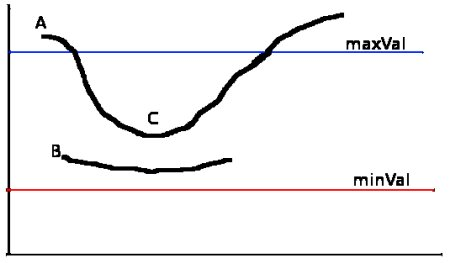
\includegraphics[width=.65\linewidth]{images/Development/chap3/hysteresis.jpg}
\caption{Hysteresis Thresholding. Source: \cite{canny_opencv_nodate}}
\label{fig: hysteresis}
\end{figure}

As an example, edge A, whose gradient intensity exceeds the maxVal threshold, is classified as safe. Edge C, even though it falls below the maxVal threshold, is connected to edge A and is thus recognized as a valid edge. However, edge B, despite having intensity above the minVal threshold and being located in the same region as edge C, is not connected to any safe edge. Therefore, it is discarded.

In conclusion, it is emphasized that the Canny filtering method is a robust and efficient approach for obtaining edges in images, based on mathematically optimized models for this purpose. This procedure is structured into several stages that converge to the final result. Initially, noise is reduced by applying a Gaussian filter, followed by the calculation of the intensity gradient, which allows for determining the direction and magnitude at each pixel. Next, the non-maximum suppression phase aims to eliminate pixels that are not at the peak of the gradient, contributing to the accuracy of the method. Subsequently, thresholds (minVal and maxVal) are defined to distinguish genuine edges, ensuring the effectiveness of the technique. Finally, the implementation of hysteresis edge tracking determines that edges with gradient intensity within the threshold range are considered true only if connected to "safe edge" pixels. Thus, the Canny algorithm emerges as a comprehensive and reliable strategy for edge detection and discrimination in digital images, providing high precision and performance to the process.

\section{ Systems}\label{section: System}

 Systems, characterized as systems built around microprocessors and designed to control a specific function or a range of functions, have played a crucial role in various technological applications. Incorporating hardware and software components, they are not intended to be programmed for direct end-user consumption, unlike personal computers, as their programming is focused on executing a specific task, although it allows for different options and choices \cite{heath2002embedded}.

This type of system exhibits an innate ability to interact with the physical world, processing and responding to signals, whether they are analog or digital, thus becoming the cornerstone of numerous contemporary innovations. The functional core of these systems is anchored in the Central Processing Unit (CPU), which coordinates all system activities. Simultaneously, a micro-controller, by integrating various peripheral components into a single circuit, contributes to the efficiency and economy of these systems \cite{peckol2019embedded}.

The importance of  systems is unequivocally evident in their extensive range of applications, spanning from common household appliances to the sophisticated Internet of Things (IoT). This breadth of use illustrates their crucial and indispensable role in contemporary technological infrastructure. In the context of this work, one of the employed  systems was the Jetson Nano\textsuperscript{\textregistered}, as seen in Figure \ref{fig:jetson}. This system, specifically designed for image processing, stands out particularly when applied in image recognition using \acrfull{cnn}, confirming its specialization and effectiveness in this domain \cite{nvidia_jetson_2019}.

\begin{figure}[ht!]
\centering
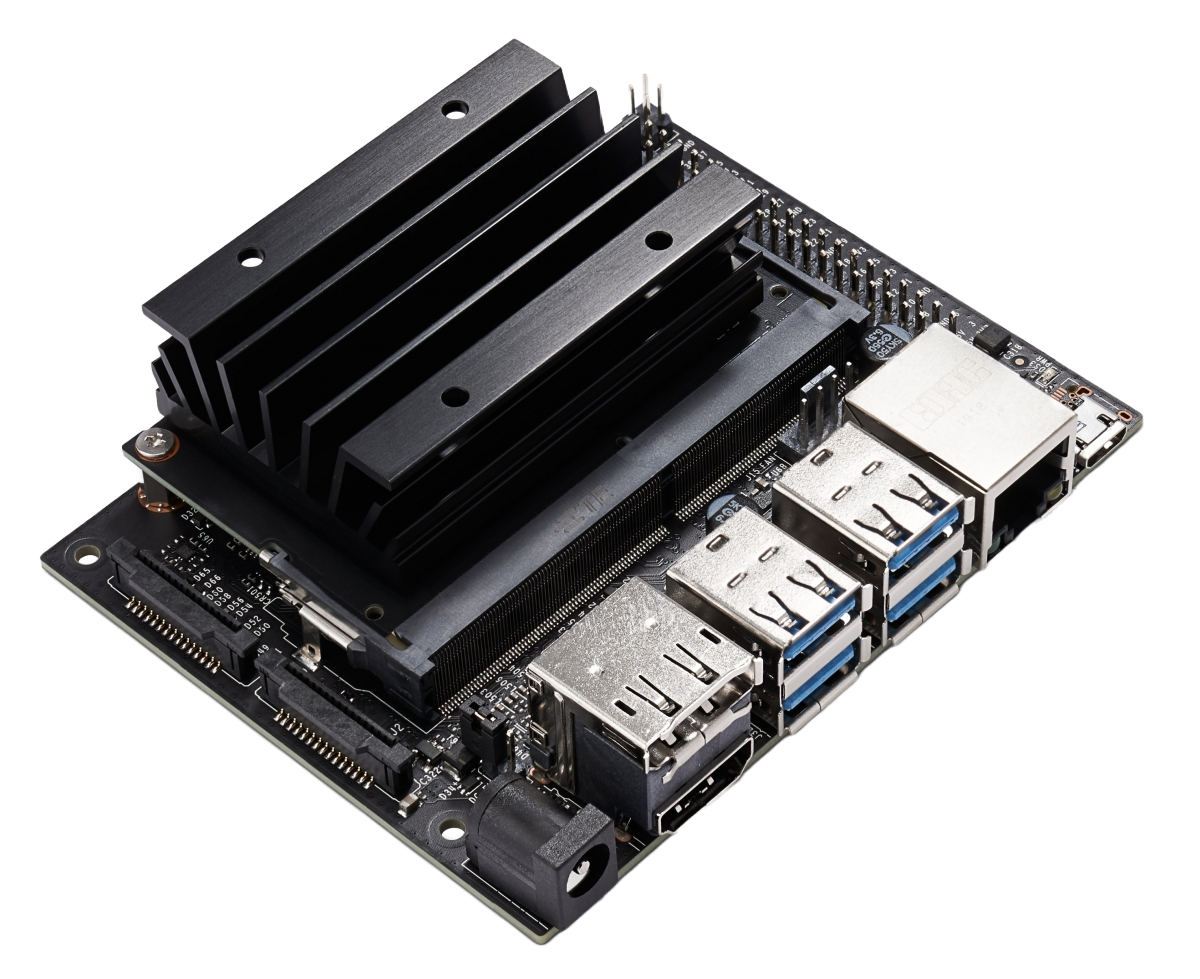
\includegraphics[width=.65\linewidth]{images/Development/chap3/JetsonNano.png}
\caption{Graphical representation of Jetson Nano\textsuperscript{\textregistered}. Source: \cite{nvidia_jetson_2019}}
\label{fig: jetson}
\end{figure}

Another hardware used was the U3-36L0XC-C\textsuperscript{\textregistered} camera, manufactured by IDS\textsuperscript{\textregistered}. This camera is capable of automatically producing high-quality images and videos, efficiently adapting to variations in object distance and unfavorable lighting conditions. It is equipped with the CMOS AR1335\textsuperscript{\textregistered} sensor, manufactured by Onsemi\textsuperscript{\textregistered}, which has a resolution of 13.10 megapixels. This sensor, operating based on rolling shutter technology, has a resolution of 4200 x 3120 pixels and a pixel size of 1.1µm, offering a frame rate of 20.0 fps, ensuring the capture of detailed and accurate images of the captured object \cite{ids_imaging_development_systemsu3-36l0xc_2023}.


\begin{figure}[ht!]
\centering
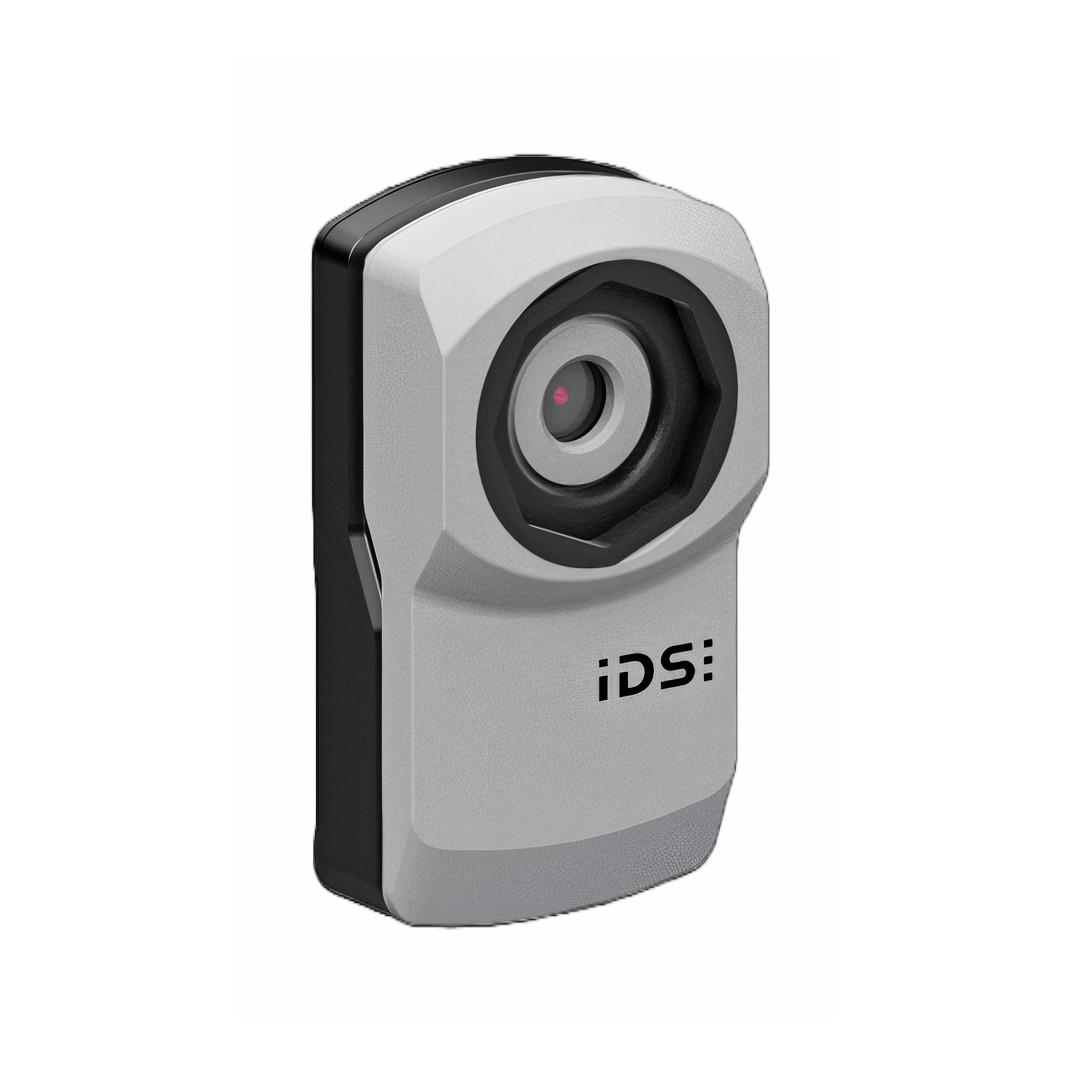
\includegraphics[width=.65\linewidth]{images/Development/chap3/IDS_CAMERA.png}
\caption{Graphical representation of Jetson Nano\textsuperscript{\textregistered}. Source: \cite{nvidia_jetson_2019}}
\label{fig: jetson}
\end{figure}

In this work, the adopted methodology for the data flow begins with the image capture process by the U3-36L0XC-C\textsuperscript{\textregistered} camera. Subsequently, these images are transmitted to the Jetson Nano\textsuperscript{\textregistered} hardware via a wired connection, ensuring the quality and integrity of the transferred data.

In the next stage, these images undergo treatment and processing on the Jetson Nano\textsuperscript{\textregistered}. After completing this crucial step, the processed data is transferred via the HTTP protocol to the server located at Mofreitas.

Finally, with the data stored on the server, it becomes possible to make it available for access and manipulation through a Restful \acrfull{api}\footnote{An Application Programming Interface (API) provides an abstraction for a problem and specifies how clients should interact with software components that implement a solution to that problem. APIs define reusable building blocks that allow incorporating modular functionality into end applications \cite{reddy2011api}}. This enables the integration of this data into the web platform, allowing it to be used for multiple purposes. Thus, the present methodology outlines an effective balance between data transmission security and efficient integration among the various elements of the system. A broader view of the data flow can be seen in Figure \ref{fig:simpleModelOfTheDataProcess}.

\begin{figure}[h!]
    \centering
    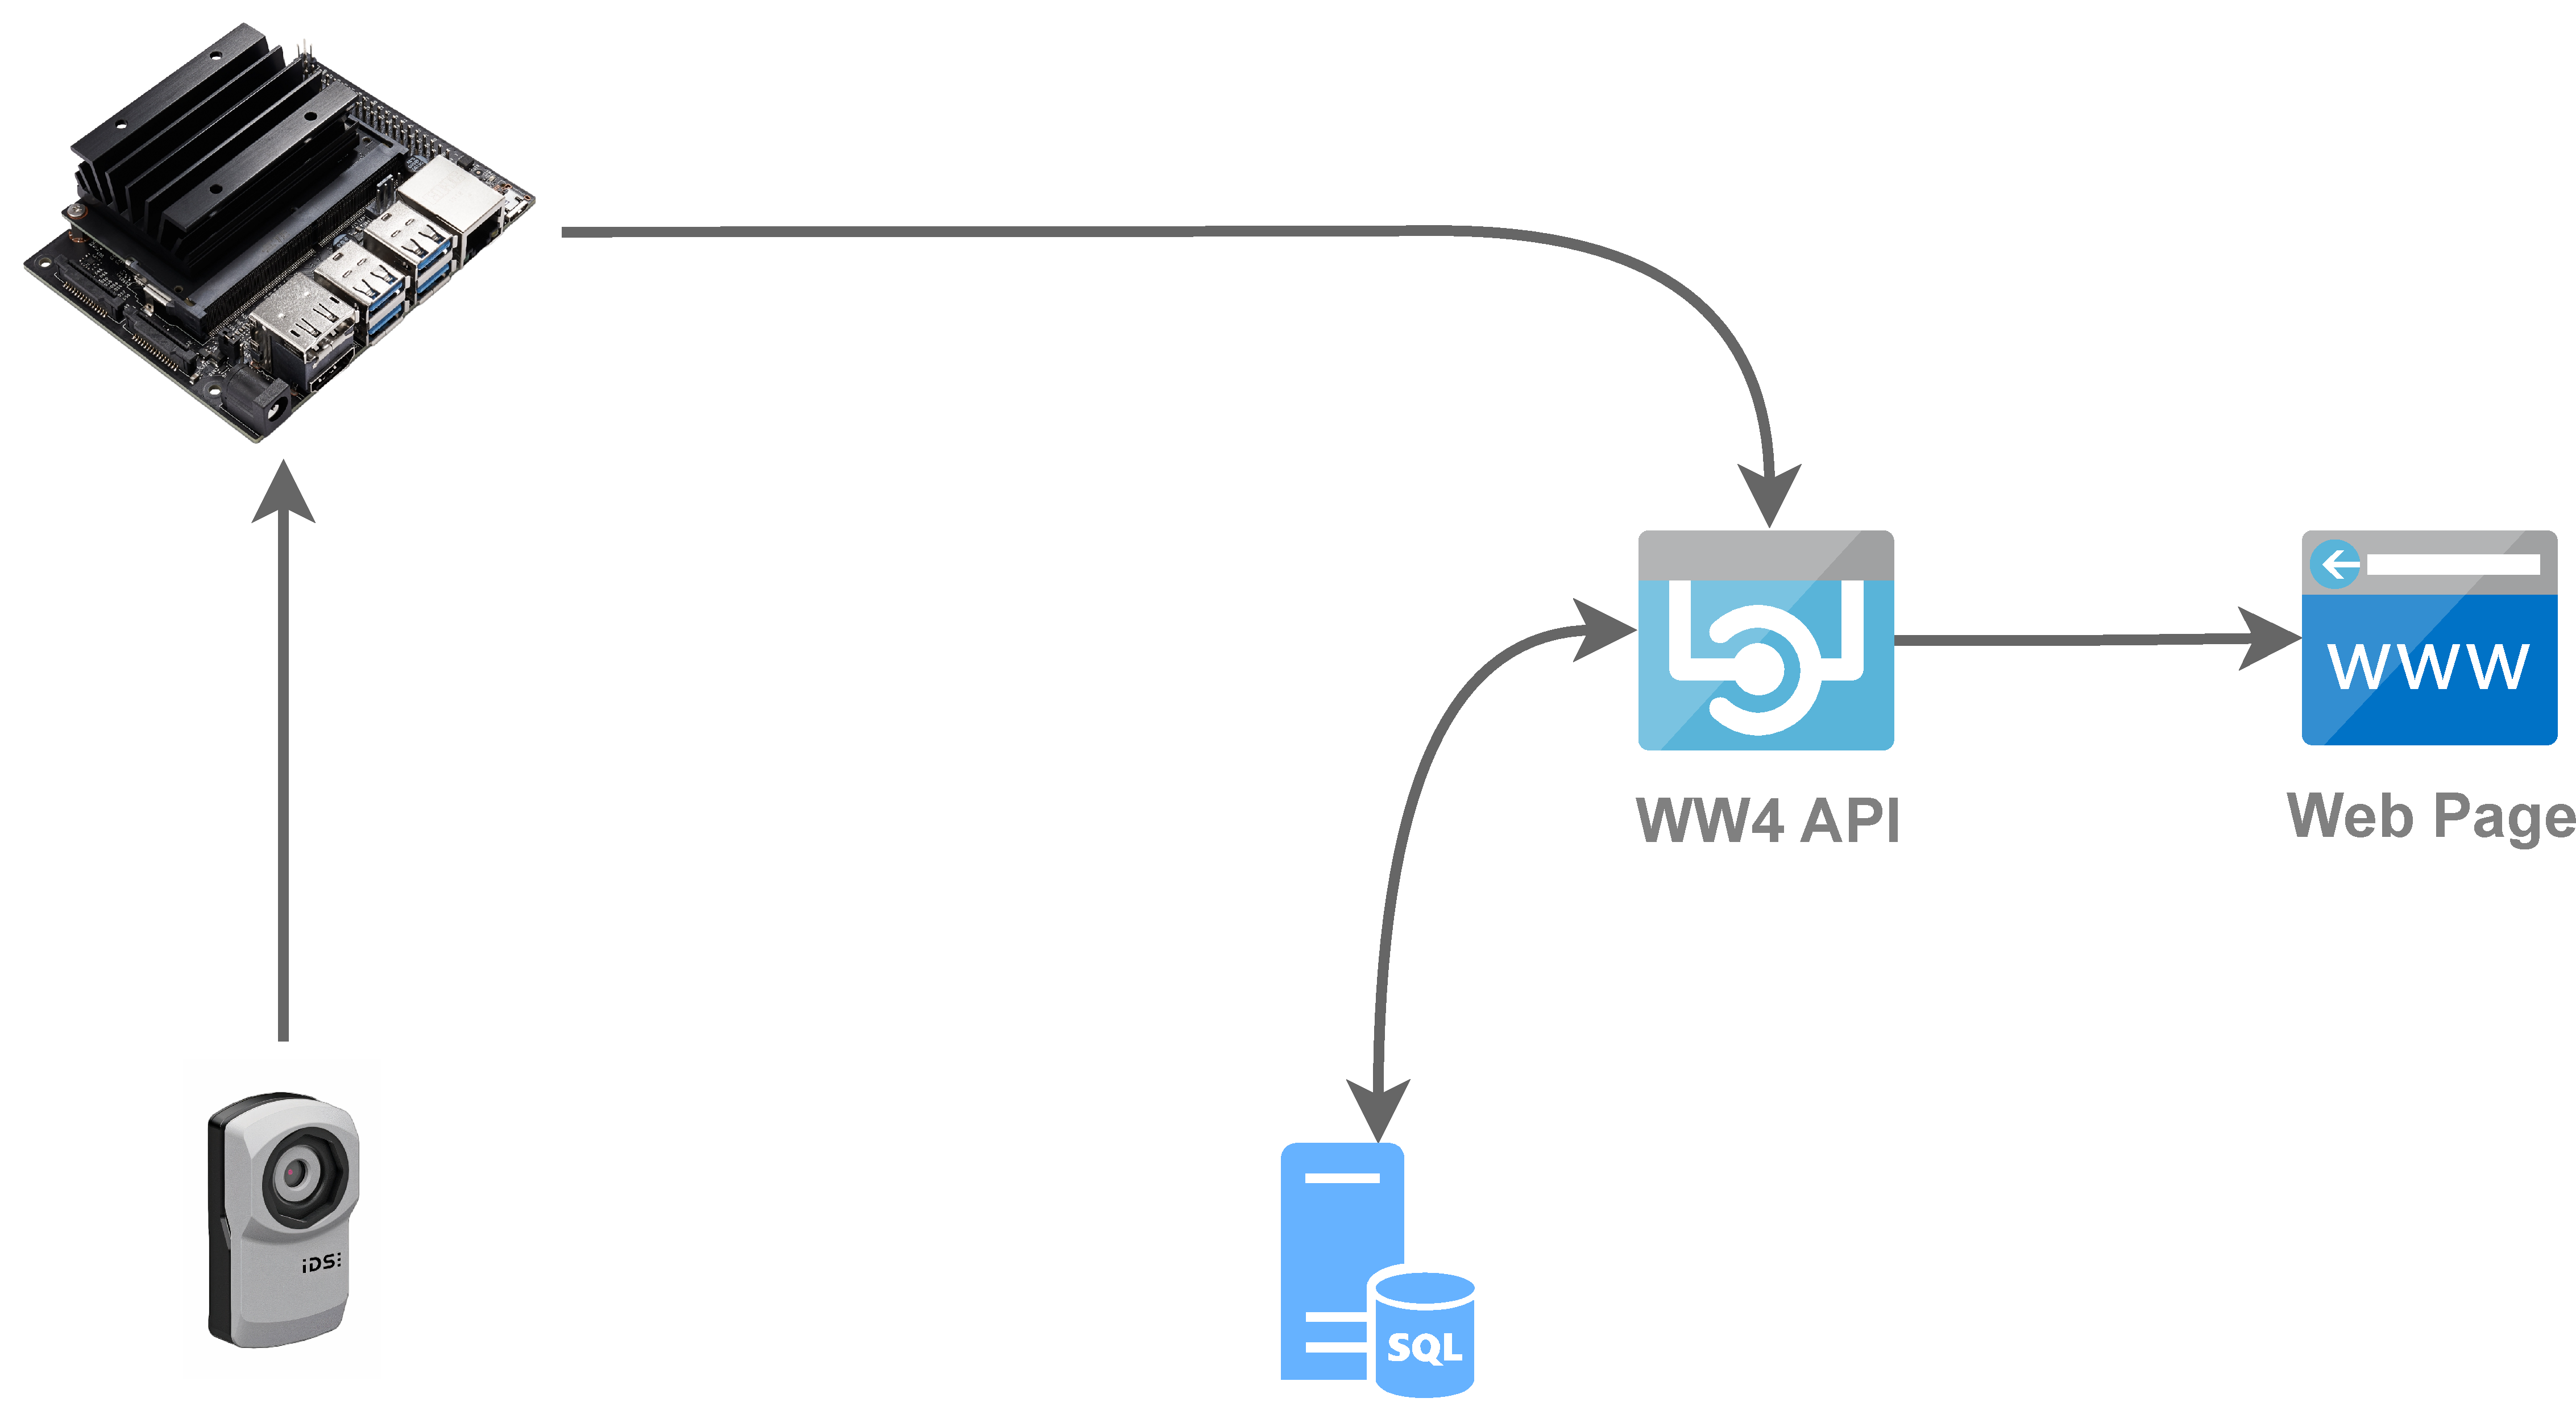
\includegraphics[width=.65\linewidth]{images/Development/chap3/LeftOver.pdf}
    \caption{Simplified Model of Communication between  Systems and the WW4 Server.}
    \label{fig:simpleModelOfTheDataProcess}
\end{figure}

\section{Communication Between Devices}\label{section:comunication}

Establishing robust methodologies for communication between devices is an essential component in this project, which, in turn, requires a deep understanding of the technologies integrated in this stage.

At the core of this project is the Orion-LD GE, a software specialized in managing data from various devices, which provides a standardized communication interface between these devices, the NGSI-LD API. This interface, based on the REST model\footnote{A REST (Representational State Transfer) API is a set of conventions for building and interacting with web services. It uses HTTP methods to manipulate data and is generally used to allow communication between different systems in an efficient and standardized way. A REST API is stateless, that is, each request from the client to the server must contain all the information necessary to understand and fulfill the request, without the server having to remember previous requests \cite{Mark2011}.}, It uses the HTTP protocol for communication, making it efficient and practical. However, a peculiarity of this interface is that it only supports data that can be serialized in JSON format, thus standardizing and unifying communication between devices. However, this characteristic imposes some limitations, such as the inability to transmit binary data. Therefore, it is established that the adopted communication method must not only follow the Restful model but also be able to serialize data in JSON format in order to maximize the effectiveness of the interaction between devices \cite{etsi2023}.

However, it is important to note that the U3-36L0XC-C camera and the Jetson Nano, mentioned earlier in Section \ref{section: System}, adopt a different communication approach. Specifically, the U3-36L0XC-C camera communicates with the Jetson Nano through serialized ports, ensuring a constant flow of data \cite{ids_imaging_development_systemsu3-36l0xc_2023}. On the other hand, the Jetson Nano has the ability to establish direct communication with the server using the MQTT protocol\footnote{MQTT (Message Queuing Telemetry Transport) is an open and efficient messaging protocol designed for bandwidth-constrained environments such as Machine-to-Machine (M2M) and Internet of Things (IoT) where a compact code representation is required \cite{banks2019mqtt}.}. The latter proves particularly useful in Internet of Things contexts, where energy efficiency and bandwidth optimization are vital considerations.


Another technology employed in this project is the \acrfull{wsgi} application, which essentially serves as the backend service built in Python. This application interacts primarily with three entities: the  system Jetson, the Orion-LD Context Broker, and the Email server. To communicate with the first two entities, Jetson and Orion-LD, the HTTP protocol is used. For communication with the Email server, a different network protocol is employed. The \acrfull{smtp} protocol allows the \acrfull{wsgi} application to establish direct and reliable communication with the Email server, which is especially useful for sending transactional emails. These emails may include registration confirmations, password change notifications, and other relevant communications for users. Thus, each entity has a specific communication method, contributing to the overall efficiency of the project.


\section{Conceptual Data Model}\label{section:conceptulaDataModel}

The design of a data model constitutes a fundamental step in this project. However, for proper execution, it is essential to formulate a methodology. In this perspective, the definition of a series of structured procedures becomes necessary to guide and provide a framework for its implementation. Thus, in this section, we propose to elucidate the methodology for this procedure while highlighting the tools that have been strategically employed during the process.

The digitization of the business world relies on one crucial step: the transfer of real-world ideas into the digital realm. In other words, the creation of a Conceptual Data Model (\acrshort{cdm}). This phase encompasses the abstraction and representation of data relevant to an organization's reality, transforming the real world into a processable and understandable form for the digital system. When executed rigorously and appropriately, the \acrshort{cdm} has the potential to significantly enhance system functionality and efficiency. Moreover, it contributes to error minimization, provides better alignment with user needs, and offers the ability to effectively adapt to changing user demands. Last but not least, a well-implemented \acrshort{cdm} can reduce the inherent costs of system development and maintenance \cite{Batra1995}.

Therefore, the starting point for creating a data model is to acquire a comprehensive understanding of the processes. To illustrate, Figure \ref{fig:MofreitasWorkflow} provides an amplified visualization of the workflow. Simplifying, it all starts with a project design request from the client. As the specifications are detailed by the client, the design department strives to create drafts until the desired outcome is achieved by the client.

\begin{figure}[H]
    \centering
    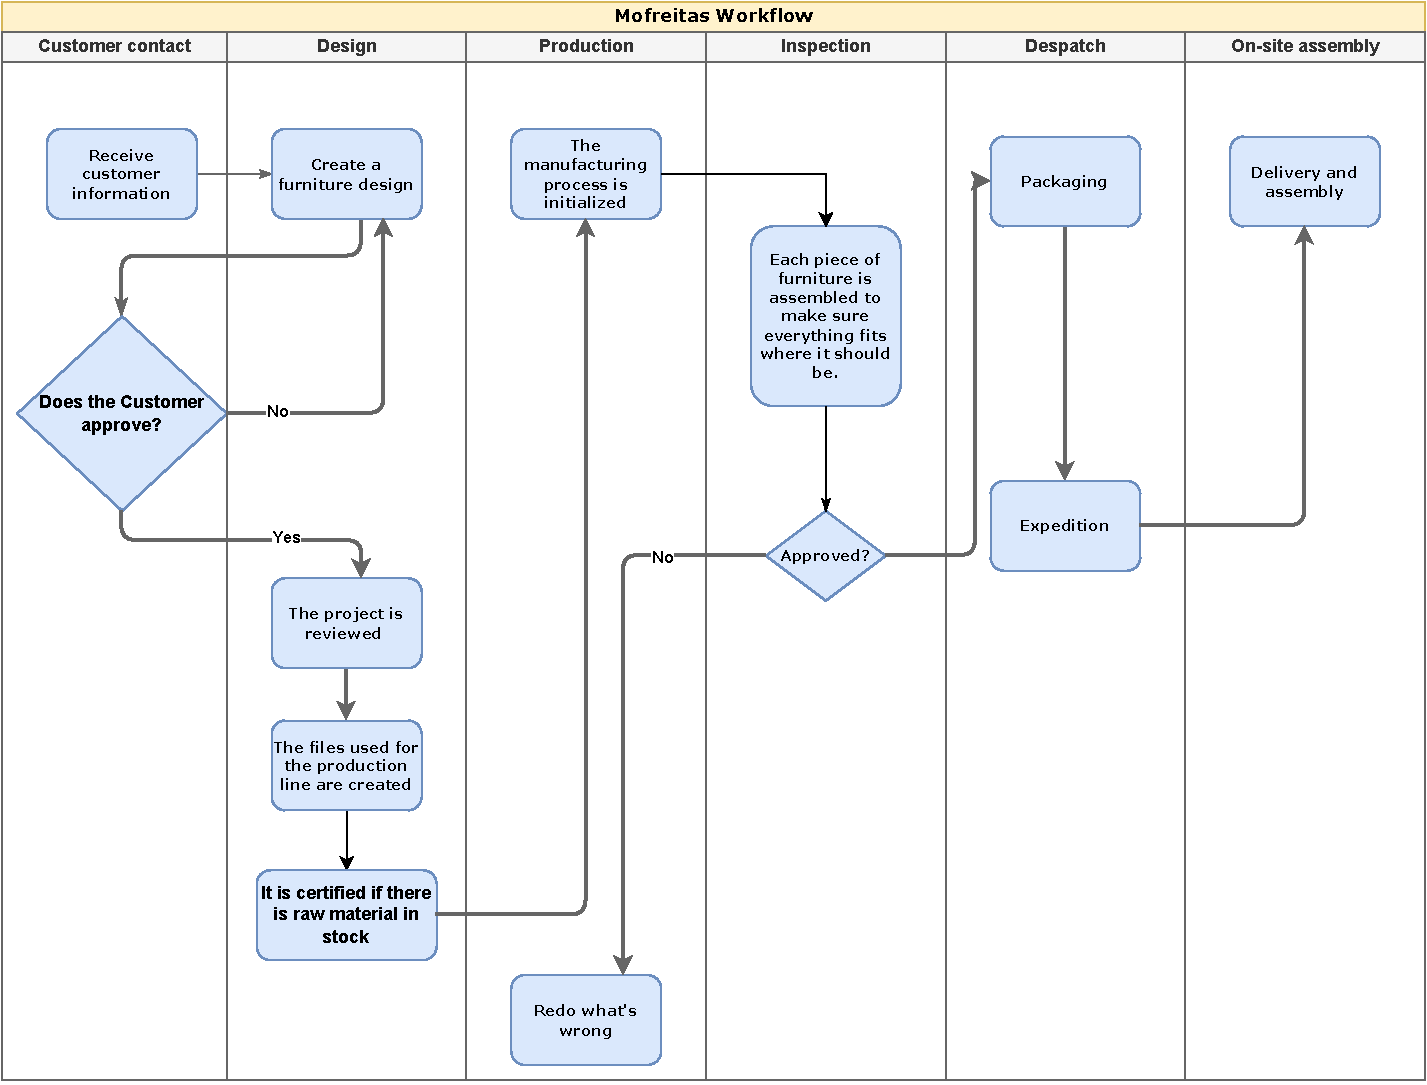
\includegraphics[width=.98\linewidth]{images/Development/chap3/Mofreitas Process.pdf}
    \caption{An abstraction of the process flow that unfolds during the execution of a project at Mofreitas.}
    \label{fig:MofreitasWorkflow}
\end{figure}

Subsequently, the design department comes into play to verify the availability of resources in the factory and proceeds to create the necessary files for the production of wooden furniture. This documentation includes cutting lists, files for \acrfull{cam}, 3D images, and files for \acrfull{cad}. Once this stage is completed, the project is forwarded to the factory, initiating the manufacturing phase. This stage involves a myriad of machines and procedures, whose combination may be unique to each project.


Once all the pieces are manufactured, the furniture is sent to the assembly line. At this stage, a pre-assembly takes place to identify possible manufacturing errors or any missing components. Once the integrity of the product is confirmed, it proceeds to the packaging phase, which is carried out with the aim of optimizing space during transportation.

Finally, after the dispatch of the pieces, the culmination of the process is the reassembly of the project at the client's location, marking the completion of the service provided by Mofreitas.

In the context of the technologies applied in this project, as mentioned in Section \ref{section:comunication}, we can identify the concrete application of certain key concepts. The Fiware\textsuperscript{\textregistered} platform, for example, utilizes context entities, which represent both physical objects and logical concepts, to build a data model that serves as a bridge between the real world and the digital world. Each entity is composed of a set of attributes and metadata for these attributes, which are employed to mirror their real-world properties. Building upon these context entities, the NGSI-LD API provides a data model for context information, as well as interfaces for data exchange and information on how to acquire such data. Crucially, all these components are encoded in \gls{json} format, establishing a universally readable and flexible standard for data structuring and manipulation \cite{etsi2023}.

In the pursuit of effective machine-to-machine interaction, the incorporation of semantics into entities becomes indispensable, as data takes on a specific meaning that is reflected in the real world \cite{Li2009}. Thus, data needs to be contextualized to convey its intrinsic meaning. This fact led \textcite{Chen1976} to publish the academic work "The entity-relationship model," which was one of the precursors to the current \acrfull{erd}. In the project at hand, the creation of a data model was necessary to represent the production process of Mofreitas, mapping entities in a logical and physical domain. However, the first step of this methodology involved the development of an \acrshort{erd}, a powerful tool in the realm of data modeling that can visualize entities, their interrelationships, and attributes, thus constructing a conceptual representation of the interactions between different entities in the system. This diagram can be viewed in Figure \ref{fig:conceptualModel}.

\begin{figure}[!ht]
    \centering
    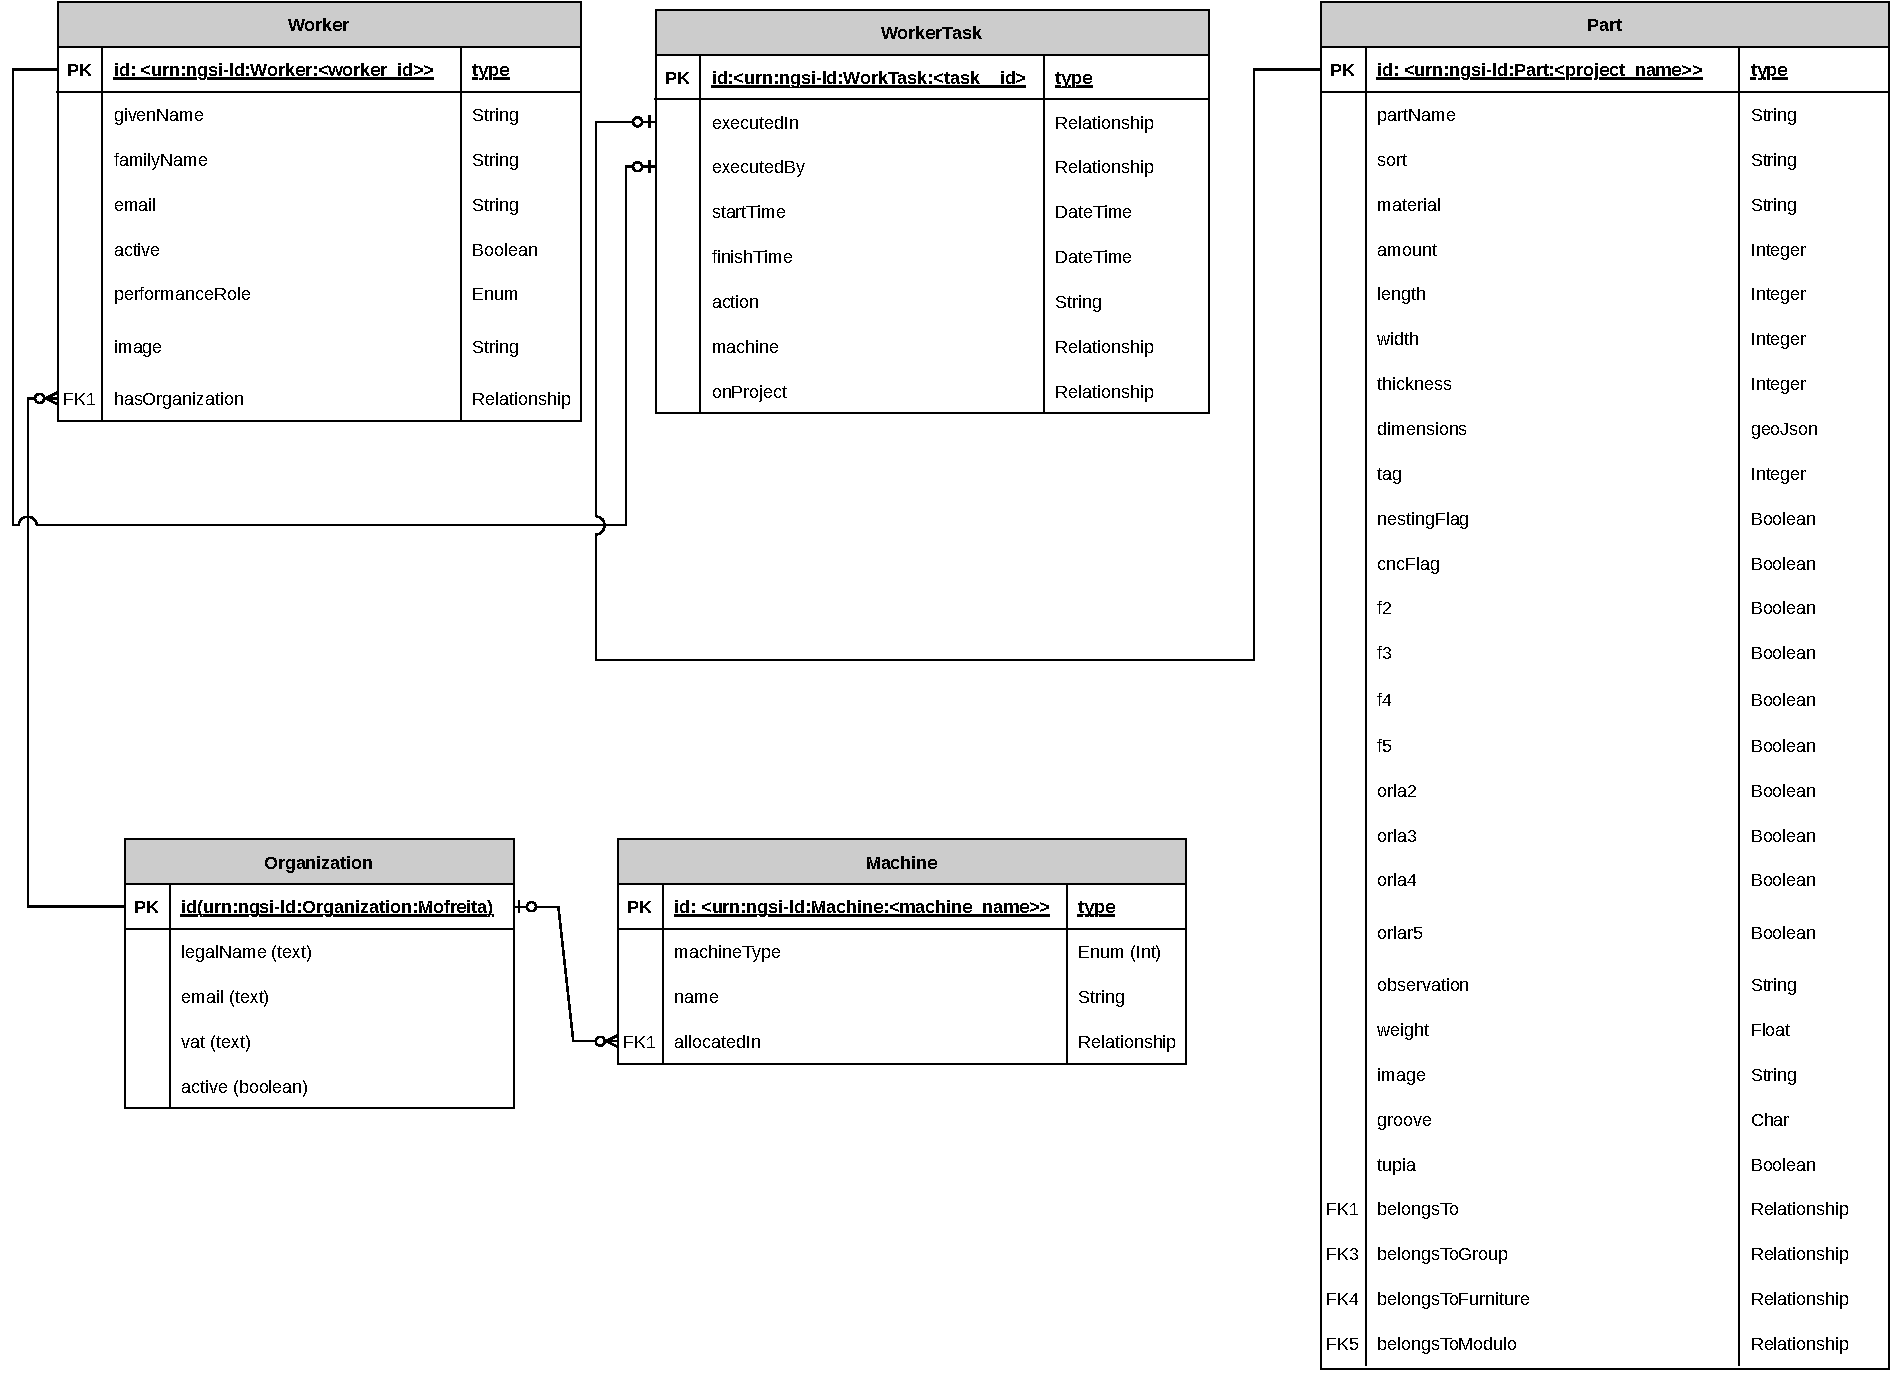
\includegraphics[width=.65\linewidth]{images/Development/chap3/WoodWork- Part 1.pdf}
    \caption{Development of the \acrfull{erd} for Mofreitas Carpentry Part One.}
    \label{fig:conceptualModel-part1}
\end{figure}

\begin{figure}[!ht]
    \centering
    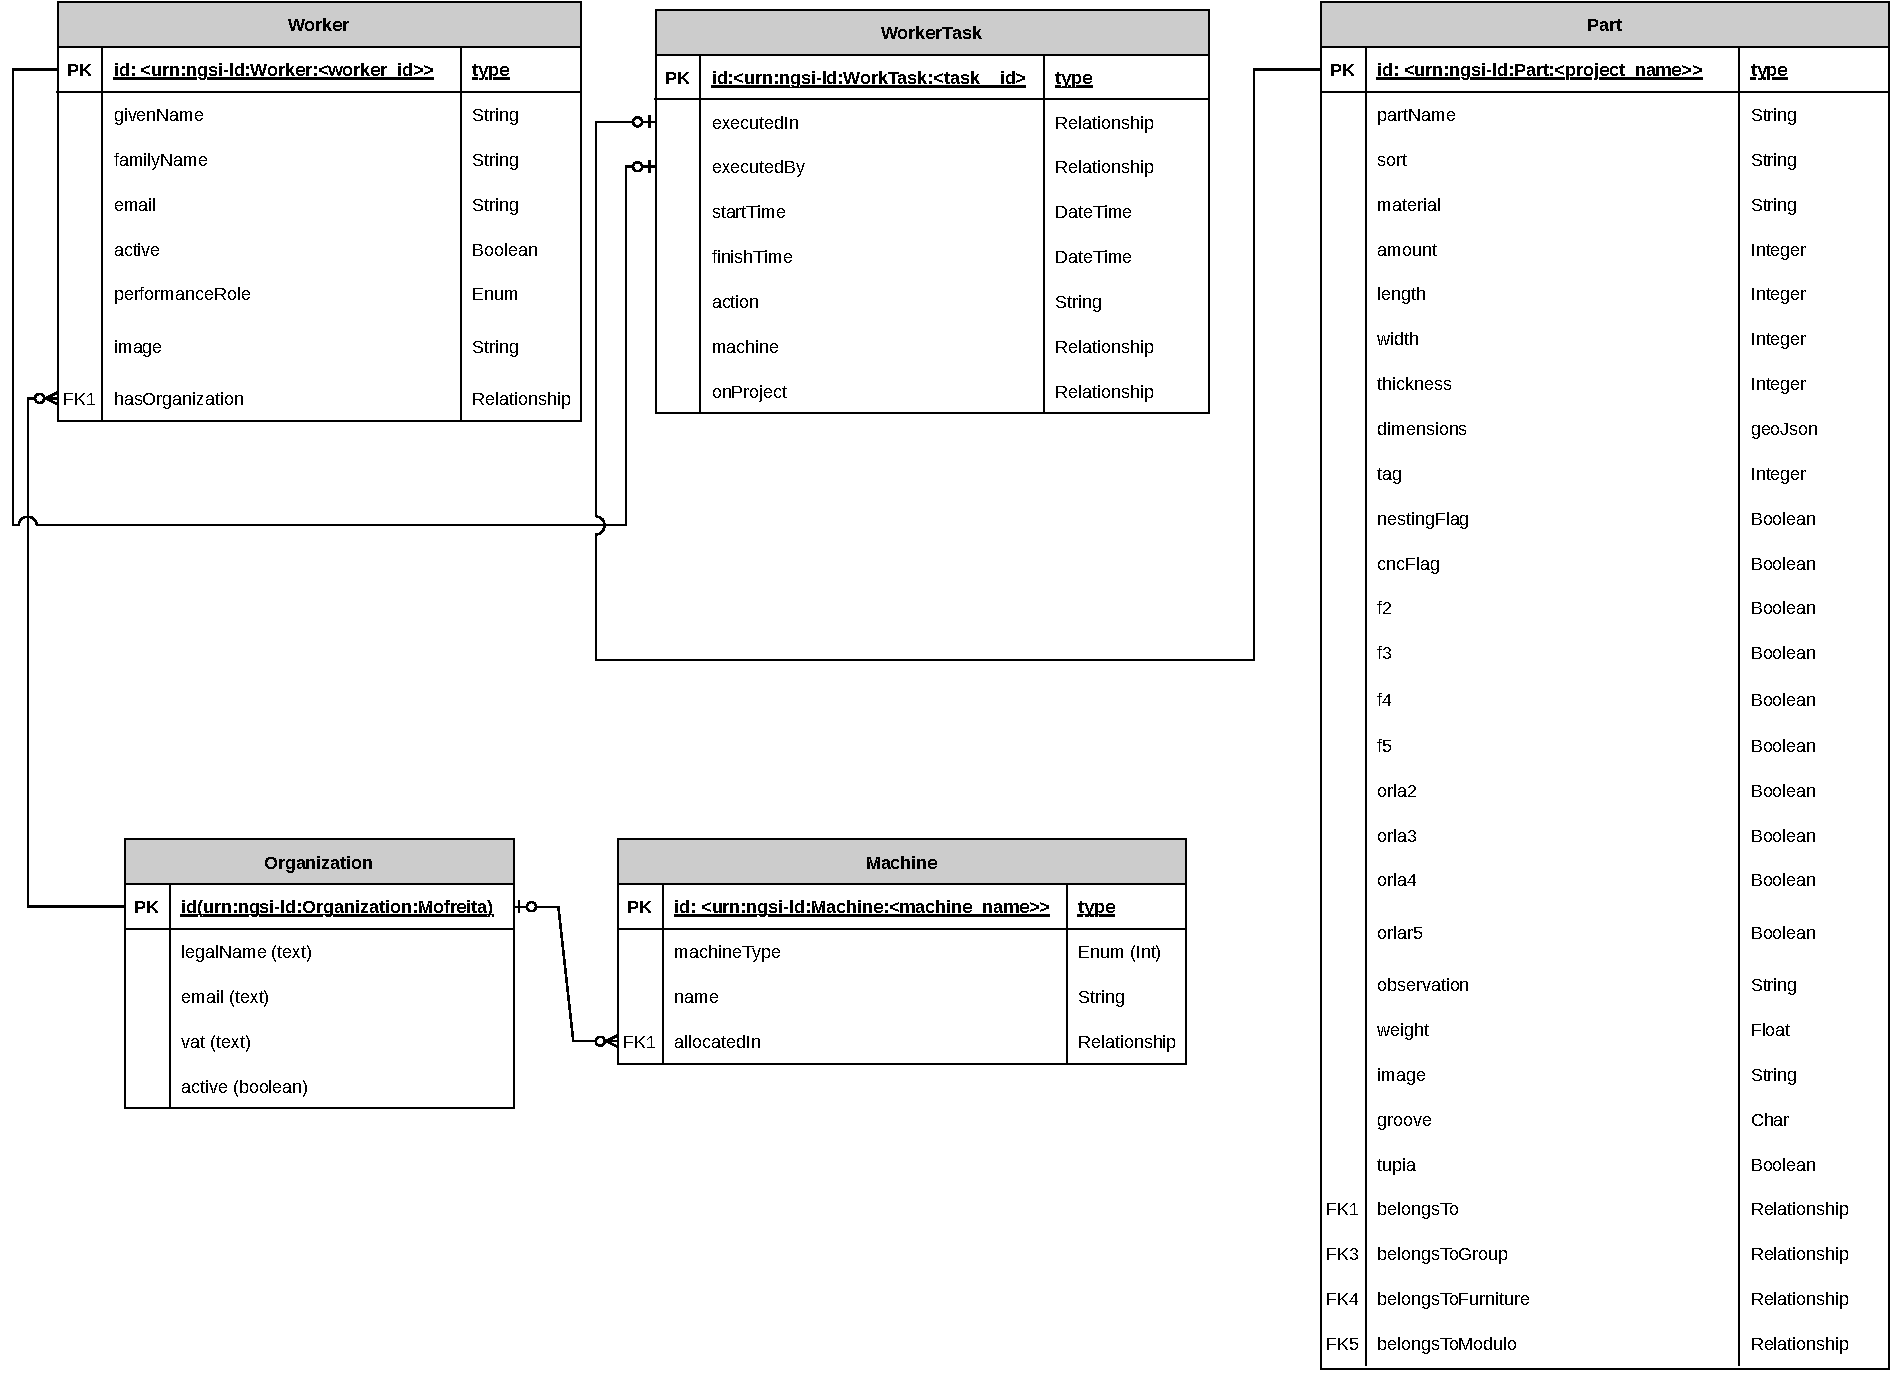
\includegraphics[width=.65\linewidth]{images/Development/chap3/WoodWork- Part 1.pdf}
    \caption{Development of the \acrfull{erd} for Mofreitas Carpentry Part Two.}
    \label{fig:conceptualModel-part2}
\end{figure}

Figure \ref{fig:conceptualModel} provides an overview of the developed data model. However, to offer a more detailed visual perspective, but it has been divided into the following two parts \ref{fig:conceptualModel-part2} and \ref{fig:conceptualModel-part1}.

\begin{figure}[H]
    \centering
    \includegraphics[width=.82\linewidth]{images/Development/chap3/WoodWork.drawio.pdf}
    \caption{Development of the \acrfull{erd} for Mofreitas Carpentry.}
    \label{fig:conceptualModel}
\end{figure}


After defining the overall view of the elements through the \acrfull{erd}, the subsequent step involves the development of the schemas.\footnote{The visualizations of the schemas created for the project can be perused and scrutinized in the GitHub repository, accessible through the following link: \href{https://github.com/More-Collaborative-Laboratory/ww4zero}{GitHub Repository}
.}. These schemas serve as the basis for creating future context files \cite{fiware_ngsi-ld_nodate}. The code \ref{code:model} exemplifies this idea.

To summarize the process, the development of a conceptual data model involves a series of interconnected steps. Initially, the crucial phase involves a comprehensive understanding of Mofreitas' business plan. With this deep understanding, it is possible to transpose the entities - both physical and logical - into an \acrfull{erd}. Subsequently, as a direct result of this modeling, there is a demand for the creation of schemas. These schemas will be applied in the future as context information in the NGSI-LD API.

\begin{listing}[H]
\begin{minted}[linenos, frame=single]{yaml}
schemas:
  project:
    type: object
    title: Project
    description: Contains the information of a project
    properties:
      id:
        description: Unique identifier of the project
        example: urn:ngsi-ld:Project:[name]
        format: uri
        type: string
        x-ngsi:
          type: Property
      type:
        description: NGSI Entity type
        enum:
          - Project
        type: string
        x-ngsi:
          type: Property
      name:
        description: Project name
        example: MUEBLE-WC
        type: string
        x-ngsi:
          model: https://schema.org/name
          type: Property
          uri: https://schema.org/name
          uri-prefix: https://schema.org/
    // Other attributes ...
    required:
      - name
      - hasBudget
\end{minted}
\caption{In the presented example, a project is created with an attribute of type "Property" for the "name" attribute.}
\label{code:model}
\end{listing}
\section{Database}\label{section:mmDataBase}

In this section, we provide details about the databases used in the context of this work, specifying their fundamental characteristics. The objective is to clarify the criteria underlying the selection of these data management systems. Additionally, we discuss the methodology employed for storing the information.

In a comprehensive manner, both relational and non-relational databases were chosen for utilization. Regarding relational databases, MySQL\textsuperscript{\textregistered} \cite{mysql_ab_mysql_2023} and PostgreSQL\textsuperscript{\textregistered} \cite{postgresql_global_postgresql_2023} were selected. On the other hand, in relation to non-relational databases, Redis\textsuperscript{\textregistered}\cite{redis_redis_2023} and MongoDB\textsuperscript{\textregistered} \cite{mongodb_inc_d2023} were adopted. Each of these databases was selected based on their specific characteristics and suitability to the dataset and functional requirements of the project.

Numerous companies dealing with significant amounts of unstructured data have progressively adopted the use of NoSQL databases \cite{Leavitt2010}. This trend is partly due to the fact that NoSQL databases, which acronym stands for "Not Only SQL," encompass a diverse range of data management systems. Unlike traditional relational systems, these databases do not primarily rely on tabular structures and often do not use SQL as the primary language for data manipulation \cite{moniruzzaman2013nosql}.

This shift towards NoSQL systems has been driven by scalability demands imposed by large-scale modern applications, such as Facebook, Amazon, and Twitter, which require data distribution across a wide range of servers. These demands challenge the limitations of traditional relational database systems, which are designed under the assumption that all operations belonging to a specific transaction must be executed by a single database node. Therefore, the emergence of NoSQL databases presents an appropriate response to meet these contemporary scalability needs \cite{moniruzzaman2013nosql}.

According to the comparative study conducted by \textcite{Cornelia2015}, MongoDB\textsuperscript{\textregistered} exhibited substantial advantages in terms of processing speed compared to MySQL\textsuperscript{\textregistered}. Specifically, MongoDB was faster in search, insertion, and deletion operations. This makes MongoDB a more efficient choice for dynamic applications with significant data processing demands. However, as demonstrated by \textcite{ron2015no}, MongoDB\textsuperscript{\textregistered} has security issues similar to those found in MySQL. \textcite{Kumar2017} propose a methodology that enables secure storage of information in NoSQL databases. However, despite the apparent effectiveness of this methodology, it was not applied in this project as the software responsible for managing this information was entirely developed by \acrshort{fiware}\textsuperscript{\textregistered}.


However, structured databases such as MySQL\textsuperscript{\textregistered} and PostgreSQL\textsuperscript{\textregistered} also have their advantages. One of the most relevant advantages is technological maturity, especially in terms of security, where these systems have a long history of problem-solving. Additionally, these types of databases are better equipped to handle more complex data queries and data encryption \cite{nance2013nosql}. Another significant factor for enhanced security in the SQL model is the fact that transactions are ACID (atomicity, consistency, isolation, durability). ACID compliance is crucial for business data and mission-critical applications. MySQL, for example, uses components like the InnoDB storage engine to adhere to the ACID model, protecting data from corruption and exceptions caused by crashes and malfunctions. ACID-compliant features eliminate the need for custom consistency checking and crash recovery mechanisms. In scenarios like user registration, where multiple records need to be inserted into various tables, ACID transactions ensure that either all insertions succeed or none of them occur. This prevents inconsistent states that could be problematic for authentication \cite{mohamed2014relational}.

As mentioned earlier, MongoDB\textsuperscript{\textregistered} has the ability to manage multiple connections and support unstructured data. This allows it to process information in a highly dynamic manner and adapt to each individual case. This characteristic makes MongoDB\textsuperscript{\textregistered} particularly suitable for the ORION-LD\textsuperscript{\textregistered} software, considering that this service needs to connect to multiple IoT devices and deal with a wide variety of data. Another NoSQL solution used is Redis. Although often referred to as a database due to its data persistence capability, Redis\textsuperscript{\textregistered} is not a traditional relational database. Redis\textsuperscript{\textregistered} is an open-source in-memory data structure storage solution used as a database, cache, message broker, and streaming engine \cite{redis_redis_2023}. In the application at hand, Redis is used for parallel processing. In this scenario, it receives tasks from task producers and forwards them to task consumers. It is used for tasks such as sending emails and processing images with AI \acrshort{ai}.


\section{Security}\label{section:security}


In this section, the aim is to explain the security tools and methodology used. In general terms, the employed tools are the Keyrock GE from \acrshort{fiware}\textsuperscript{\textregistered}, as well as Django\textsuperscript{\textregistered}, an internal security framework. The Django\textsuperscript{\textregistered} framework, complemented with some Python\textsuperscript{\textregistered} libraries, allows for the expansion of its security functionalities.

The security system of \acrshort{fiware}\textsuperscript{\textregistered} stands out for its robustness and efficiency. The platform makes use of the Keyrock Identity Management (IDM) in conjunction with the Wilma PEP Proxy\textsuperscript{\textregistered} for access control. This software configuration employs the OAuth2 protocol for user and application authentication. While it is a highly effective system for limiting internal user access to the network and the system, Keyrock does not allow direct registration of external clients. Therefore, all registrations must be conducted by an internal administrator. Although this situation addresses most issues associated with intelligent applications, it is a limiting factor. Taking this into consideration, the \acrshort{wsgi} application was developed as an external application that facilitates access to \acrshort{fiware}\textsuperscript{\textregistered}'s internal resources. This situation can be visualized in Figure \ref{fig:security}.


\begin{figure}[H]
    \centering
    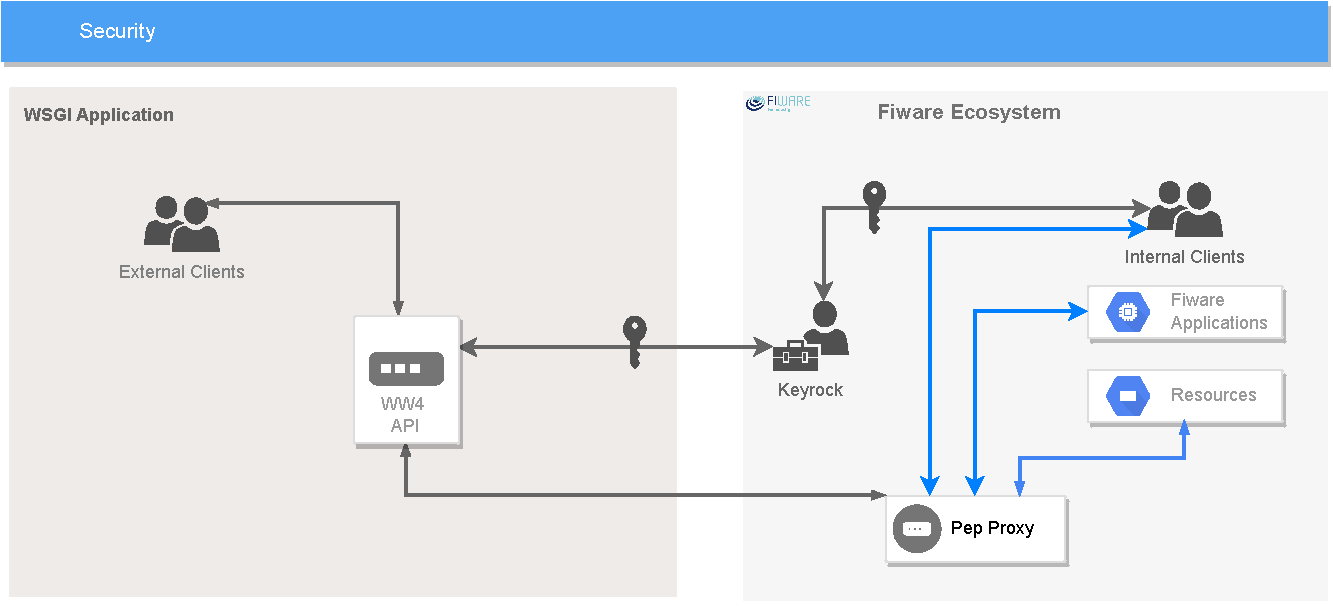
\includegraphics[width=.95\linewidth]{images/Development/chap3/Security.pdf}
    \caption{Development of the \acrfull{erd} for Mofreitas Carpentry.}
    \label{fig:security}
\end{figure}


\section{Web Server}\label{section:fileSharing-webserver}

In this section, the methodology used for the selection of the web server and the chosen software to fulfill this function are discussed.

Three fundamental criteria were established for choosing a web server for the project:

\begin{enumerate}
    \item Scalability: The ability of the web server to handle an increasing number of requests and expand to accommodate this growth is an essential attribute.
    \item Performance: The efficiency and speed at which the web server processes requests and delivers responses are crucial for the overall system performance.
    \item Reliability: The expectation that the web server operates in a stable and reliable manner, with minimal failures or interruptions, is indispensable for the project's operations continuity.
\end{enumerate}

There are several widely used servers to act as a web server. Among these, the ones that commonly stand out in real-world applications are Nginx and the Apache HTTP Server \cite{rob_mccool_apache_2023}.

The comparative study conducted by \textcite{nguyen2017comparative} identified Nginx as a superior option to Apache for environments with a high number of concurrent processes. Nginx is not limited to being a web server; it also offers Reverse-Proxy and Load Balancer functionalities. In this regard, studies conducted by the authors \cite{Chi2012} highlighted that Nginx is a notable alternative to the HAProxy Reverse-Proxy and Load Balancer \cite{willy_tarreau_haproxy_nodate}.

Furthermore, \textcite{Pramono2018} concluded that even when Nginx uses its Open Source version with default configuration, it delivers competitive results compared to HAProxy.

Based on these factors, Nginx was chosen for this project due to its versatility and notable performance compared to reference software, significantly contributing to its scalability. Additionally, Nginx, being a widely recognized solution in the market, provides a high level of reliability.

\section{File Sharing}\label{section:fileSharing}

In this section, the focus is on elucidating the methodology implemented for file sharing, as well as the tools employed in this process. The central premise is the need to have access to projects and their corresponding files from any location on the factory floor. A crucial aspect for efficient project monitoring is the ability to access both the project management platform and the files associated with a specific project. With this goal in mind, a file sharing strategy was developed, the details and necessary tools of which will be presented below.

One of the central software components in the sharing strategy is Syncthing\textsuperscript{\textregistered} \cite{jakob_borg_syncthing_nodate}. Syncthing is a decentralized, open-source, peer-to-peer file synchronization application.\footnote{Peer-to-peer (P2P) refers to the concept of an entity acting as a "Servent", a term used in peer-to-peer networks. The word "Servent" is an artificial combination of the first syllable of the term "server" ("Serv-") and the second syllable of the term "client" ("-ent"). In other words, it is a computer network architecture in which each computer acts as both a client and a server. This allows resources to be shared directly between nodes without the need for a centralized server \cite{Schollmeier2001}.}. This software is available for various operating systems. The goal of Syncthing is to provide a reliable and secure way to synchronize files across multiple computers. It works by creating a shared folder, which exists on both the computers of the users connected to the Syncthing network and the server. In this way, all the data contained in this folder is kept synchronized between the parties, ensuring that all information is consistently up to date. See Figure \ref{fig:syncFiles}.

\begin{figure}[!ht]
    \centering
    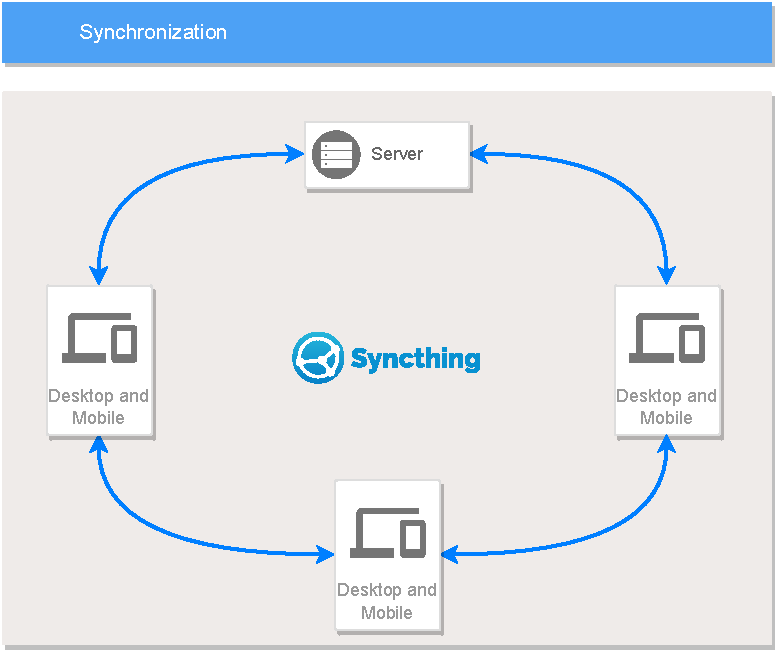
\includegraphics[width=.65\linewidth]{images/Development/chap3/Syncronization.pdf}
    \caption{Representation of the synchronization scheme implemented to share files from each Mofreitas employee's computer system with the Web Server.}
    \label{fig:syncFiles}
\end{figure}

In order for the files stored on the web server to be properly represented in the WW4 API in the JSON format, so that they can be interpreted by the web application, it is essential that the API can identify and catalog any new file that is added to the shared folder. This detection allows the API to indicate the correct location of the file and provide access to it.

This strategy involves the use of a third-party software, which is responsible for continuously monitoring the shared folder. This software is programmed to observe file system events, meaning that each time a file is created, deleted, or modified, the software informs the API about the change and indicates the location of the affected file.

Based on this information, the API is responsible for storing this data in a database, in order to reflect the exact structure of the shared folder. To ensure that the data model is efficient and robust, aligning with the objectives of this system, the \acrfull{mptt} algorithm was chosen. This algorithm plays the role of associating each data with a node in an interconnected network, similar to the structure of a file system (see Figure \ref{fig:syncFilesMPTT}). Thus, modifications or deletions of higher-level nodes trigger changes throughout the chain of lower-level nodes, ensuring the correct updating of the system's structure.

\begin{figure}[!ht]
    \centering
    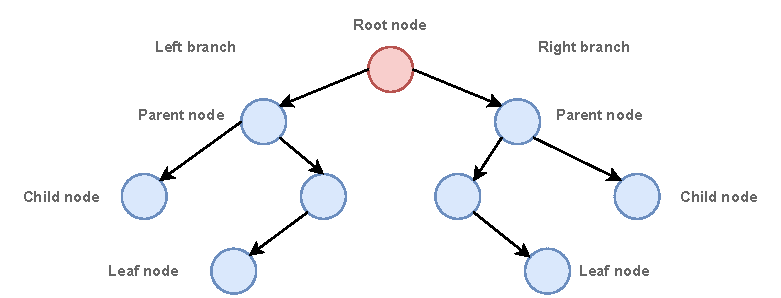
\includegraphics[width=.65\linewidth]{images/Development/chap3/MPTT.pdf}
    \caption{Representation of the \acrfull{mptt} structure. Adapted from: \cite{srihithnavigating}.}
    \label{fig:syncFilesMPTT}
\end{figure}



\section{Traceability of a Project}\label{section:ProjectTraceability}

In this section, the methods employed to ensure project traceability are discussed. As illustrated in Figure \ref{fig:MofreitasWorkflow}, after the project design is approved by the client, various files are generated. Among them, cutting lists are notable as they contain all the relevant information for the project components, including items such as hardware and wooden pieces.

This information is of fundamental importance as it facilitates the population of a database with the components that are part of the project and other tertiary elements associated with a specific project.

With this in mind, an application has been developed that supervises the creation of cutting lists and extracts all the relevant information for project monitoring. This application represents the first step towards the automated insertion of project data into the database.

With this data available, the operator then takes over the tracking of the components. Using a control interface, they can identify the component to be produced and record the start of production by pressing the "Start" button. This procedure allows for the collection of information about the time required for component production and which components are in production. Figure \ref{fig:projectTraceability} demonstrates the process involved.

\begin{figure}[!ht]
    \centering
    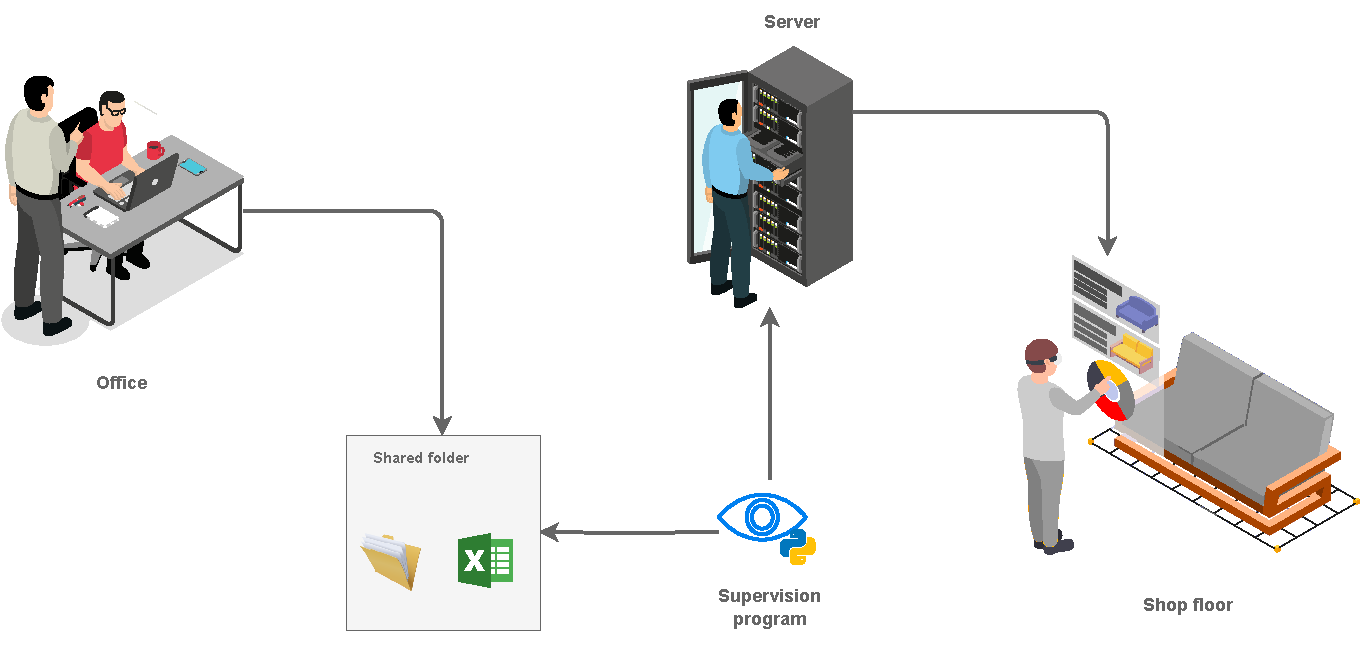
\includegraphics[width=.75\linewidth]{images/Development/chap3/File sharing.pdf}
    \caption{The initial project data is harvested from a shared project folder by a supervisory program. This data is then stored on a central server. Subsequently, it can be accessed from the factory floor using interfaces, for instance the Human-Machine Interface (HMI), to direct the production processes.}
    \label{fig:projectTraceability}
\end{figure}

Although this methodology may not seem particularly innovative, it represents a significant advancement compared to the traditional process. Previously, control was done manually, with each operator recording their activities on paper sheets. The lack of integration with the overall system could result in insufficient communication, which sometimes led to two workers performing the same task, causing waste of time and material.

Furthermore, the old system did not allow the client or the design team to have easy access to the current state of the project. With the data now available in a database, it is possible to develop a web application that presents this information to both the client and the design team, displaying the current state of a specific project.


\section{Traceability of a Leftover}\label{section:LeftoverTraceability}


A leftover represents a residue resulting from the wood manufacturing process, which may or may not have commercial value. In this section, the methodology applied to track a commercially valuable leftover and the tools involved in this procedure are detailed.

The employed strategy is based on the use of a leftover sorting table. This table is responsible for determining the dimensions and type of wood of the leftover and records this information in the database.

The attributes of the leftover, such as width, length, and material type, are identified through image processing, using, for example, the Canny filter mentioned in section \ref{subsection:Canny-edge-detection}. After these steps, a QR code is attached to the leftover, and its corresponding information is recorded in the database.

Developing a data model for material type detection is not a trivial task. It requires training with a large set of images to develop a reliable model. Thus, it was decided to implement a semi-supervised system that is constantly evolving. The images are presented to the factory operator, who assesses and corrects, if necessary, the system's detections. Upon reaching a sufficient volume of data, the software development team is responsible for retraining the model. When the network is considered sufficiently reliable, the aim is to make the system fully autonomous.